\documentclass[11pt]{article}

    \usepackage[breakable]{tcolorbox}
    \usepackage{parskip} % Stop auto-indenting (to mimic markdown behaviour)
    
    \usepackage{iftex}
    \ifPDFTeX
    	\usepackage[T1]{fontenc}
    	\usepackage{mathpazo}
    \else
    	\usepackage{fontspec}
    \fi

    % Basic figure setup, for now with no caption control since it's done
    % automatically by Pandoc (which extracts ![](path) syntax from Markdown).
    \usepackage{graphicx}
    % Maintain compatibility with old templates. Remove in nbconvert 6.0
    \let\Oldincludegraphics\includegraphics
    % Ensure that by default, figures have no caption (until we provide a
    % proper Figure object with a Caption API and a way to capture that
    % in the conversion process - todo).
    \usepackage{caption}
    \DeclareCaptionFormat{nocaption}{}
    \captionsetup{format=nocaption,aboveskip=0pt,belowskip=0pt}

    \usepackage{float}
    \floatplacement{figure}{H} % forces figures to be placed at the correct location
    \usepackage{xcolor} % Allow colors to be defined
    \usepackage{enumerate} % Needed for markdown enumerations to work
    \usepackage{geometry} % Used to adjust the document margins
    \usepackage{amsmath} % Equations
    \usepackage{amssymb} % Equations
    \usepackage{textcomp} % defines textquotesingle
    % Hack from http://tex.stackexchange.com/a/47451/13684:
    \AtBeginDocument{%
        \def\PYZsq{\textquotesingle}% Upright quotes in Pygmentized code
    }
    \usepackage{upquote} % Upright quotes for verbatim code
    \usepackage{eurosym} % defines \euro
    \usepackage[mathletters]{ucs} % Extended unicode (utf-8) support
    \usepackage{fancyvrb} % verbatim replacement that allows latex
    \usepackage{grffile} % extends the file name processing of package graphics 
                         % to support a larger range
    \makeatletter % fix for old versions of grffile with XeLaTeX
    \@ifpackagelater{grffile}{2019/11/01}
    {
      % Do nothing on new versions
    }
    {
      \def\Gread@@xetex#1{%
        \IfFileExists{"\Gin@base".bb}%
        {\Gread@eps{\Gin@base.bb}}%
        {\Gread@@xetex@aux#1}%
      }
    }
    \makeatother
    \usepackage[Export]{adjustbox} % Used to constrain images to a maximum size
    \adjustboxset{max size={0.9\linewidth}{0.9\paperheight}}

    % The hyperref package gives us a pdf with properly built
    % internal navigation ('pdf bookmarks' for the table of contents,
    % internal cross-reference links, web links for URLs, etc.)
    \usepackage{hyperref}
    % The default LaTeX title has an obnoxious amount of whitespace. By default,
    % titling removes some of it. It also provides customization options.
    \usepackage{titling}
    \usepackage{longtable} % longtable support required by pandoc >1.10
    \usepackage{booktabs}  % table support for pandoc > 1.12.2
    \usepackage[inline]{enumitem} % IRkernel/repr support (it uses the enumerate* environment)
    \usepackage[normalem]{ulem} % ulem is needed to support strikethroughs (\sout)
                                % normalem makes italics be italics, not underlines
    \usepackage{mathrsfs}
    

    
    % Colors for the hyperref package
    \definecolor{urlcolor}{rgb}{0,.145,.698}
    \definecolor{linkcolor}{rgb}{.71,0.21,0.01}
    \definecolor{citecolor}{rgb}{.12,.54,.11}

    % ANSI colors
    \definecolor{ansi-black}{HTML}{3E424D}
    \definecolor{ansi-black-intense}{HTML}{282C36}
    \definecolor{ansi-red}{HTML}{E75C58}
    \definecolor{ansi-red-intense}{HTML}{B22B31}
    \definecolor{ansi-green}{HTML}{00A250}
    \definecolor{ansi-green-intense}{HTML}{007427}
    \definecolor{ansi-yellow}{HTML}{DDB62B}
    \definecolor{ansi-yellow-intense}{HTML}{B27D12}
    \definecolor{ansi-blue}{HTML}{208FFB}
    \definecolor{ansi-blue-intense}{HTML}{0065CA}
    \definecolor{ansi-magenta}{HTML}{D160C4}
    \definecolor{ansi-magenta-intense}{HTML}{A03196}
    \definecolor{ansi-cyan}{HTML}{60C6C8}
    \definecolor{ansi-cyan-intense}{HTML}{258F8F}
    \definecolor{ansi-white}{HTML}{C5C1B4}
    \definecolor{ansi-white-intense}{HTML}{A1A6B2}
    \definecolor{ansi-default-inverse-fg}{HTML}{FFFFFF}
    \definecolor{ansi-default-inverse-bg}{HTML}{000000}

    % common color for the border for error outputs.
    \definecolor{outerrorbackground}{HTML}{FFDFDF}

    % commands and environments needed by pandoc snippets
    % extracted from the output of `pandoc -s`
    \providecommand{\tightlist}{%
      \setlength{\itemsep}{0pt}\setlength{\parskip}{0pt}}
    \DefineVerbatimEnvironment{Highlighting}{Verbatim}{commandchars=\\\{\}}
    % Add ',fontsize=\small' for more characters per line
    \newenvironment{Shaded}{}{}
    \newcommand{\KeywordTok}[1]{\textcolor[rgb]{0.00,0.44,0.13}{\textbf{{#1}}}}
    \newcommand{\DataTypeTok}[1]{\textcolor[rgb]{0.56,0.13,0.00}{{#1}}}
    \newcommand{\DecValTok}[1]{\textcolor[rgb]{0.25,0.63,0.44}{{#1}}}
    \newcommand{\BaseNTok}[1]{\textcolor[rgb]{0.25,0.63,0.44}{{#1}}}
    \newcommand{\FloatTok}[1]{\textcolor[rgb]{0.25,0.63,0.44}{{#1}}}
    \newcommand{\CharTok}[1]{\textcolor[rgb]{0.25,0.44,0.63}{{#1}}}
    \newcommand{\StringTok}[1]{\textcolor[rgb]{0.25,0.44,0.63}{{#1}}}
    \newcommand{\CommentTok}[1]{\textcolor[rgb]{0.38,0.63,0.69}{\textit{{#1}}}}
    \newcommand{\OtherTok}[1]{\textcolor[rgb]{0.00,0.44,0.13}{{#1}}}
    \newcommand{\AlertTok}[1]{\textcolor[rgb]{1.00,0.00,0.00}{\textbf{{#1}}}}
    \newcommand{\FunctionTok}[1]{\textcolor[rgb]{0.02,0.16,0.49}{{#1}}}
    \newcommand{\RegionMarkerTok}[1]{{#1}}
    \newcommand{\ErrorTok}[1]{\textcolor[rgb]{1.00,0.00,0.00}{\textbf{{#1}}}}
    \newcommand{\NormalTok}[1]{{#1}}
    
    % Additional commands for more recent versions of Pandoc
    \newcommand{\ConstantTok}[1]{\textcolor[rgb]{0.53,0.00,0.00}{{#1}}}
    \newcommand{\SpecialCharTok}[1]{\textcolor[rgb]{0.25,0.44,0.63}{{#1}}}
    \newcommand{\VerbatimStringTok}[1]{\textcolor[rgb]{0.25,0.44,0.63}{{#1}}}
    \newcommand{\SpecialStringTok}[1]{\textcolor[rgb]{0.73,0.40,0.53}{{#1}}}
    \newcommand{\ImportTok}[1]{{#1}}
    \newcommand{\DocumentationTok}[1]{\textcolor[rgb]{0.73,0.13,0.13}{\textit{{#1}}}}
    \newcommand{\AnnotationTok}[1]{\textcolor[rgb]{0.38,0.63,0.69}{\textbf{\textit{{#1}}}}}
    \newcommand{\CommentVarTok}[1]{\textcolor[rgb]{0.38,0.63,0.69}{\textbf{\textit{{#1}}}}}
    \newcommand{\VariableTok}[1]{\textcolor[rgb]{0.10,0.09,0.49}{{#1}}}
    \newcommand{\ControlFlowTok}[1]{\textcolor[rgb]{0.00,0.44,0.13}{\textbf{{#1}}}}
    \newcommand{\OperatorTok}[1]{\textcolor[rgb]{0.40,0.40,0.40}{{#1}}}
    \newcommand{\BuiltInTok}[1]{{#1}}
    \newcommand{\ExtensionTok}[1]{{#1}}
    \newcommand{\PreprocessorTok}[1]{\textcolor[rgb]{0.74,0.48,0.00}{{#1}}}
    \newcommand{\AttributeTok}[1]{\textcolor[rgb]{0.49,0.56,0.16}{{#1}}}
    \newcommand{\InformationTok}[1]{\textcolor[rgb]{0.38,0.63,0.69}{\textbf{\textit{{#1}}}}}
    \newcommand{\WarningTok}[1]{\textcolor[rgb]{0.38,0.63,0.69}{\textbf{\textit{{#1}}}}}
    
    
    % Define a nice break command that doesn't care if a line doesn't already
    % exist.
    \def\br{\hspace*{\fill} \\* }
    % Math Jax compatibility definitions
    \def\gt{>}
    \def\lt{<}
    \let\Oldtex\TeX
    \let\Oldlatex\LaTeX
    \renewcommand{\TeX}{\textrm{\Oldtex}}
    \renewcommand{\LaTeX}{\textrm{\Oldlatex}}
    % Document parameters
    % Document title
    \title{chapter-2-1}
    
    
    
    
    
% Pygments definitions
\makeatletter
\def\PY@reset{\let\PY@it=\relax \let\PY@bf=\relax%
    \let\PY@ul=\relax \let\PY@tc=\relax%
    \let\PY@bc=\relax \let\PY@ff=\relax}
\def\PY@tok#1{\csname PY@tok@#1\endcsname}
\def\PY@toks#1+{\ifx\relax#1\empty\else%
    \PY@tok{#1}\expandafter\PY@toks\fi}
\def\PY@do#1{\PY@bc{\PY@tc{\PY@ul{%
    \PY@it{\PY@bf{\PY@ff{#1}}}}}}}
\def\PY#1#2{\PY@reset\PY@toks#1+\relax+\PY@do{#2}}

\@namedef{PY@tok@w}{\def\PY@tc##1{\textcolor[rgb]{0.73,0.73,0.73}{##1}}}
\@namedef{PY@tok@c}{\let\PY@it=\textit\def\PY@tc##1{\textcolor[rgb]{0.25,0.50,0.50}{##1}}}
\@namedef{PY@tok@cp}{\def\PY@tc##1{\textcolor[rgb]{0.74,0.48,0.00}{##1}}}
\@namedef{PY@tok@k}{\let\PY@bf=\textbf\def\PY@tc##1{\textcolor[rgb]{0.00,0.50,0.00}{##1}}}
\@namedef{PY@tok@kp}{\def\PY@tc##1{\textcolor[rgb]{0.00,0.50,0.00}{##1}}}
\@namedef{PY@tok@kt}{\def\PY@tc##1{\textcolor[rgb]{0.69,0.00,0.25}{##1}}}
\@namedef{PY@tok@o}{\def\PY@tc##1{\textcolor[rgb]{0.40,0.40,0.40}{##1}}}
\@namedef{PY@tok@ow}{\let\PY@bf=\textbf\def\PY@tc##1{\textcolor[rgb]{0.67,0.13,1.00}{##1}}}
\@namedef{PY@tok@nb}{\def\PY@tc##1{\textcolor[rgb]{0.00,0.50,0.00}{##1}}}
\@namedef{PY@tok@nf}{\def\PY@tc##1{\textcolor[rgb]{0.00,0.00,1.00}{##1}}}
\@namedef{PY@tok@nc}{\let\PY@bf=\textbf\def\PY@tc##1{\textcolor[rgb]{0.00,0.00,1.00}{##1}}}
\@namedef{PY@tok@nn}{\let\PY@bf=\textbf\def\PY@tc##1{\textcolor[rgb]{0.00,0.00,1.00}{##1}}}
\@namedef{PY@tok@ne}{\let\PY@bf=\textbf\def\PY@tc##1{\textcolor[rgb]{0.82,0.25,0.23}{##1}}}
\@namedef{PY@tok@nv}{\def\PY@tc##1{\textcolor[rgb]{0.10,0.09,0.49}{##1}}}
\@namedef{PY@tok@no}{\def\PY@tc##1{\textcolor[rgb]{0.53,0.00,0.00}{##1}}}
\@namedef{PY@tok@nl}{\def\PY@tc##1{\textcolor[rgb]{0.63,0.63,0.00}{##1}}}
\@namedef{PY@tok@ni}{\let\PY@bf=\textbf\def\PY@tc##1{\textcolor[rgb]{0.60,0.60,0.60}{##1}}}
\@namedef{PY@tok@na}{\def\PY@tc##1{\textcolor[rgb]{0.49,0.56,0.16}{##1}}}
\@namedef{PY@tok@nt}{\let\PY@bf=\textbf\def\PY@tc##1{\textcolor[rgb]{0.00,0.50,0.00}{##1}}}
\@namedef{PY@tok@nd}{\def\PY@tc##1{\textcolor[rgb]{0.67,0.13,1.00}{##1}}}
\@namedef{PY@tok@s}{\def\PY@tc##1{\textcolor[rgb]{0.73,0.13,0.13}{##1}}}
\@namedef{PY@tok@sd}{\let\PY@it=\textit\def\PY@tc##1{\textcolor[rgb]{0.73,0.13,0.13}{##1}}}
\@namedef{PY@tok@si}{\let\PY@bf=\textbf\def\PY@tc##1{\textcolor[rgb]{0.73,0.40,0.53}{##1}}}
\@namedef{PY@tok@se}{\let\PY@bf=\textbf\def\PY@tc##1{\textcolor[rgb]{0.73,0.40,0.13}{##1}}}
\@namedef{PY@tok@sr}{\def\PY@tc##1{\textcolor[rgb]{0.73,0.40,0.53}{##1}}}
\@namedef{PY@tok@ss}{\def\PY@tc##1{\textcolor[rgb]{0.10,0.09,0.49}{##1}}}
\@namedef{PY@tok@sx}{\def\PY@tc##1{\textcolor[rgb]{0.00,0.50,0.00}{##1}}}
\@namedef{PY@tok@m}{\def\PY@tc##1{\textcolor[rgb]{0.40,0.40,0.40}{##1}}}
\@namedef{PY@tok@gh}{\let\PY@bf=\textbf\def\PY@tc##1{\textcolor[rgb]{0.00,0.00,0.50}{##1}}}
\@namedef{PY@tok@gu}{\let\PY@bf=\textbf\def\PY@tc##1{\textcolor[rgb]{0.50,0.00,0.50}{##1}}}
\@namedef{PY@tok@gd}{\def\PY@tc##1{\textcolor[rgb]{0.63,0.00,0.00}{##1}}}
\@namedef{PY@tok@gi}{\def\PY@tc##1{\textcolor[rgb]{0.00,0.63,0.00}{##1}}}
\@namedef{PY@tok@gr}{\def\PY@tc##1{\textcolor[rgb]{1.00,0.00,0.00}{##1}}}
\@namedef{PY@tok@ge}{\let\PY@it=\textit}
\@namedef{PY@tok@gs}{\let\PY@bf=\textbf}
\@namedef{PY@tok@gp}{\let\PY@bf=\textbf\def\PY@tc##1{\textcolor[rgb]{0.00,0.00,0.50}{##1}}}
\@namedef{PY@tok@go}{\def\PY@tc##1{\textcolor[rgb]{0.53,0.53,0.53}{##1}}}
\@namedef{PY@tok@gt}{\def\PY@tc##1{\textcolor[rgb]{0.00,0.27,0.87}{##1}}}
\@namedef{PY@tok@err}{\def\PY@bc##1{{\setlength{\fboxsep}{\string -\fboxrule}\fcolorbox[rgb]{1.00,0.00,0.00}{1,1,1}{\strut ##1}}}}
\@namedef{PY@tok@kc}{\let\PY@bf=\textbf\def\PY@tc##1{\textcolor[rgb]{0.00,0.50,0.00}{##1}}}
\@namedef{PY@tok@kd}{\let\PY@bf=\textbf\def\PY@tc##1{\textcolor[rgb]{0.00,0.50,0.00}{##1}}}
\@namedef{PY@tok@kn}{\let\PY@bf=\textbf\def\PY@tc##1{\textcolor[rgb]{0.00,0.50,0.00}{##1}}}
\@namedef{PY@tok@kr}{\let\PY@bf=\textbf\def\PY@tc##1{\textcolor[rgb]{0.00,0.50,0.00}{##1}}}
\@namedef{PY@tok@bp}{\def\PY@tc##1{\textcolor[rgb]{0.00,0.50,0.00}{##1}}}
\@namedef{PY@tok@fm}{\def\PY@tc##1{\textcolor[rgb]{0.00,0.00,1.00}{##1}}}
\@namedef{PY@tok@vc}{\def\PY@tc##1{\textcolor[rgb]{0.10,0.09,0.49}{##1}}}
\@namedef{PY@tok@vg}{\def\PY@tc##1{\textcolor[rgb]{0.10,0.09,0.49}{##1}}}
\@namedef{PY@tok@vi}{\def\PY@tc##1{\textcolor[rgb]{0.10,0.09,0.49}{##1}}}
\@namedef{PY@tok@vm}{\def\PY@tc##1{\textcolor[rgb]{0.10,0.09,0.49}{##1}}}
\@namedef{PY@tok@sa}{\def\PY@tc##1{\textcolor[rgb]{0.73,0.13,0.13}{##1}}}
\@namedef{PY@tok@sb}{\def\PY@tc##1{\textcolor[rgb]{0.73,0.13,0.13}{##1}}}
\@namedef{PY@tok@sc}{\def\PY@tc##1{\textcolor[rgb]{0.73,0.13,0.13}{##1}}}
\@namedef{PY@tok@dl}{\def\PY@tc##1{\textcolor[rgb]{0.73,0.13,0.13}{##1}}}
\@namedef{PY@tok@s2}{\def\PY@tc##1{\textcolor[rgb]{0.73,0.13,0.13}{##1}}}
\@namedef{PY@tok@sh}{\def\PY@tc##1{\textcolor[rgb]{0.73,0.13,0.13}{##1}}}
\@namedef{PY@tok@s1}{\def\PY@tc##1{\textcolor[rgb]{0.73,0.13,0.13}{##1}}}
\@namedef{PY@tok@mb}{\def\PY@tc##1{\textcolor[rgb]{0.40,0.40,0.40}{##1}}}
\@namedef{PY@tok@mf}{\def\PY@tc##1{\textcolor[rgb]{0.40,0.40,0.40}{##1}}}
\@namedef{PY@tok@mh}{\def\PY@tc##1{\textcolor[rgb]{0.40,0.40,0.40}{##1}}}
\@namedef{PY@tok@mi}{\def\PY@tc##1{\textcolor[rgb]{0.40,0.40,0.40}{##1}}}
\@namedef{PY@tok@il}{\def\PY@tc##1{\textcolor[rgb]{0.40,0.40,0.40}{##1}}}
\@namedef{PY@tok@mo}{\def\PY@tc##1{\textcolor[rgb]{0.40,0.40,0.40}{##1}}}
\@namedef{PY@tok@ch}{\let\PY@it=\textit\def\PY@tc##1{\textcolor[rgb]{0.25,0.50,0.50}{##1}}}
\@namedef{PY@tok@cm}{\let\PY@it=\textit\def\PY@tc##1{\textcolor[rgb]{0.25,0.50,0.50}{##1}}}
\@namedef{PY@tok@cpf}{\let\PY@it=\textit\def\PY@tc##1{\textcolor[rgb]{0.25,0.50,0.50}{##1}}}
\@namedef{PY@tok@c1}{\let\PY@it=\textit\def\PY@tc##1{\textcolor[rgb]{0.25,0.50,0.50}{##1}}}
\@namedef{PY@tok@cs}{\let\PY@it=\textit\def\PY@tc##1{\textcolor[rgb]{0.25,0.50,0.50}{##1}}}

\def\PYZbs{\char`\\}
\def\PYZus{\char`\_}
\def\PYZob{\char`\{}
\def\PYZcb{\char`\}}
\def\PYZca{\char`\^}
\def\PYZam{\char`\&}
\def\PYZlt{\char`\<}
\def\PYZgt{\char`\>}
\def\PYZsh{\char`\#}
\def\PYZpc{\char`\%}
\def\PYZdl{\char`\$}
\def\PYZhy{\char`\-}
\def\PYZsq{\char`\'}
\def\PYZdq{\char`\"}
\def\PYZti{\char`\~}
% for compatibility with earlier versions
\def\PYZat{@}
\def\PYZlb{[}
\def\PYZrb{]}
\makeatother


    % For linebreaks inside Verbatim environment from package fancyvrb. 
    \makeatletter
        \newbox\Wrappedcontinuationbox 
        \newbox\Wrappedvisiblespacebox 
        \newcommand*\Wrappedvisiblespace {\textcolor{red}{\textvisiblespace}} 
        \newcommand*\Wrappedcontinuationsymbol {\textcolor{red}{\llap{\tiny$\m@th\hookrightarrow$}}} 
        \newcommand*\Wrappedcontinuationindent {3ex } 
        \newcommand*\Wrappedafterbreak {\kern\Wrappedcontinuationindent\copy\Wrappedcontinuationbox} 
        % Take advantage of the already applied Pygments mark-up to insert 
        % potential linebreaks for TeX processing. 
        %        {, <, #, %, $, ' and ": go to next line. 
        %        _, }, ^, &, >, - and ~: stay at end of broken line. 
        % Use of \textquotesingle for straight quote. 
        \newcommand*\Wrappedbreaksatspecials {% 
            \def\PYGZus{\discretionary{\char`\_}{\Wrappedafterbreak}{\char`\_}}% 
            \def\PYGZob{\discretionary{}{\Wrappedafterbreak\char`\{}{\char`\{}}% 
            \def\PYGZcb{\discretionary{\char`\}}{\Wrappedafterbreak}{\char`\}}}% 
            \def\PYGZca{\discretionary{\char`\^}{\Wrappedafterbreak}{\char`\^}}% 
            \def\PYGZam{\discretionary{\char`\&}{\Wrappedafterbreak}{\char`\&}}% 
            \def\PYGZlt{\discretionary{}{\Wrappedafterbreak\char`\<}{\char`\<}}% 
            \def\PYGZgt{\discretionary{\char`\>}{\Wrappedafterbreak}{\char`\>}}% 
            \def\PYGZsh{\discretionary{}{\Wrappedafterbreak\char`\#}{\char`\#}}% 
            \def\PYGZpc{\discretionary{}{\Wrappedafterbreak\char`\%}{\char`\%}}% 
            \def\PYGZdl{\discretionary{}{\Wrappedafterbreak\char`\$}{\char`\$}}% 
            \def\PYGZhy{\discretionary{\char`\-}{\Wrappedafterbreak}{\char`\-}}% 
            \def\PYGZsq{\discretionary{}{\Wrappedafterbreak\textquotesingle}{\textquotesingle}}% 
            \def\PYGZdq{\discretionary{}{\Wrappedafterbreak\char`\"}{\char`\"}}% 
            \def\PYGZti{\discretionary{\char`\~}{\Wrappedafterbreak}{\char`\~}}% 
        } 
        % Some characters . , ; ? ! / are not pygmentized. 
        % This macro makes them "active" and they will insert potential linebreaks 
        \newcommand*\Wrappedbreaksatpunct {% 
            \lccode`\~`\.\lowercase{\def~}{\discretionary{\hbox{\char`\.}}{\Wrappedafterbreak}{\hbox{\char`\.}}}% 
            \lccode`\~`\,\lowercase{\def~}{\discretionary{\hbox{\char`\,}}{\Wrappedafterbreak}{\hbox{\char`\,}}}% 
            \lccode`\~`\;\lowercase{\def~}{\discretionary{\hbox{\char`\;}}{\Wrappedafterbreak}{\hbox{\char`\;}}}% 
            \lccode`\~`\:\lowercase{\def~}{\discretionary{\hbox{\char`\:}}{\Wrappedafterbreak}{\hbox{\char`\:}}}% 
            \lccode`\~`\?\lowercase{\def~}{\discretionary{\hbox{\char`\?}}{\Wrappedafterbreak}{\hbox{\char`\?}}}% 
            \lccode`\~`\!\lowercase{\def~}{\discretionary{\hbox{\char`\!}}{\Wrappedafterbreak}{\hbox{\char`\!}}}% 
            \lccode`\~`\/\lowercase{\def~}{\discretionary{\hbox{\char`\/}}{\Wrappedafterbreak}{\hbox{\char`\/}}}% 
            \catcode`\.\active
            \catcode`\,\active 
            \catcode`\;\active
            \catcode`\:\active
            \catcode`\?\active
            \catcode`\!\active
            \catcode`\/\active 
            \lccode`\~`\~ 	
        }
    \makeatother

    \let\OriginalVerbatim=\Verbatim
    \makeatletter
    \renewcommand{\Verbatim}[1][1]{%
        %\parskip\z@skip
        \sbox\Wrappedcontinuationbox {\Wrappedcontinuationsymbol}%
        \sbox\Wrappedvisiblespacebox {\FV@SetupFont\Wrappedvisiblespace}%
        \def\FancyVerbFormatLine ##1{\hsize\linewidth
            \vtop{\raggedright\hyphenpenalty\z@\exhyphenpenalty\z@
                \doublehyphendemerits\z@\finalhyphendemerits\z@
                \strut ##1\strut}%
        }%
        % If the linebreak is at a space, the latter will be displayed as visible
        % space at end of first line, and a continuation symbol starts next line.
        % Stretch/shrink are however usually zero for typewriter font.
        \def\FV@Space {%
            \nobreak\hskip\z@ plus\fontdimen3\font minus\fontdimen4\font
            \discretionary{\copy\Wrappedvisiblespacebox}{\Wrappedafterbreak}
            {\kern\fontdimen2\font}%
        }%
        
        % Allow breaks at special characters using \PYG... macros.
        \Wrappedbreaksatspecials
        % Breaks at punctuation characters . , ; ? ! and / need catcode=\active 	
        \OriginalVerbatim[#1,codes*=\Wrappedbreaksatpunct]%
    }
    \makeatother

    % Exact colors from NB
    \definecolor{incolor}{HTML}{303F9F}
    \definecolor{outcolor}{HTML}{D84315}
    \definecolor{cellborder}{HTML}{CFCFCF}
    \definecolor{cellbackground}{HTML}{F7F7F7}
    
    % prompt
    \makeatletter
    \newcommand{\boxspacing}{\kern\kvtcb@left@rule\kern\kvtcb@boxsep}
    \makeatother
    \newcommand{\prompt}[4]{
        {\ttfamily\llap{{\color{#2}[#3]:\hspace{3pt}#4}}\vspace{-\baselineskip}}
    }
    

    
    % Prevent overflowing lines due to hard-to-break entities
    \sloppy 
    % Setup hyperref package
    \hypersetup{
      breaklinks=true,  % so long urls are correctly broken across lines
      colorlinks=true,
      urlcolor=urlcolor,
      linkcolor=linkcolor,
      citecolor=citecolor,
      }
    % Slightly bigger margins than the latex defaults
    
    \geometry{verbose,tmargin=1in,bmargin=1in,lmargin=1in,rmargin=1in}
    
    

\begin{document}
    
    \maketitle
    
    

    
    Run in Google Colab

    \hypertarget{deep-learning-for-option-pricing}{%
\section{Deep Learning for Option
Pricing}\label{deep-learning-for-option-pricing}}

    \begin{tcolorbox}[breakable, size=fbox, boxrule=1pt, pad at break*=1mm,colback=cellbackground, colframe=cellborder]
\prompt{In}{incolor}{154}{\boxspacing}
\begin{Verbatim}[commandchars=\\\{\}]
\PY{k+kn}{import} \PY{n+nn}{sys}
\PY{k+kn}{import} \PY{n+nn}{math}
\PY{k+kn}{import} \PY{n+nn}{time}
\PY{k+kn}{import} \PY{n+nn}{numpy}             \PY{k}{as} \PY{n+nn}{np}
\PY{k+kn}{import} \PY{n+nn}{pandas}            \PY{k}{as} \PY{n+nn}{pd}
\PY{k+kn}{import} \PY{n+nn}{matplotlib}\PY{n+nn}{.}\PY{n+nn}{pyplot} \PY{k}{as} \PY{n+nn}{plt}

\PY{k+kn}{from} \PY{n+nn}{scipy}\PY{n+nn}{.}\PY{n+nn}{stats}             \PY{k+kn}{import} \PY{n}{norm}
\PY{k+kn}{from} \PY{n+nn}{sklearn}\PY{n+nn}{.}\PY{n+nn}{model\PYZus{}selection} \PY{k+kn}{import} \PY{n}{train\PYZus{}test\PYZus{}split}
\end{Verbatim}
\end{tcolorbox}

    \hypertarget{introduction}{%
\subsection{Introduction}\label{introduction}}

The problem of this first part of our lessons can be stated simply as
follow. Let's say, from a very general point of view, that we have a
contingent claim \(\cal{V}\) that depends on \(D\) parameters:

\[
\cal{V}(\mathbf{x}), \, \mathbf{x}=\left\{x_1,\dots, x_D \right\} \in \mathbb{R}^D
\]

We want to approximate the pricing function with a neural network.
Remember that we can always consider the NN as a sort of mapping
function

\[
\Phi : \mathbb{R}^D \rightarrow \mathbb{R}
\]

trained to compute prices given a point in $\mathbb{R}^D$
representing a particular set of parameters.

The use of a NN as a pricing functions has a number of advantages. the
first is that in this way we are able to compute efficiently thousands
of prices in a small amount of time, even when the derivative contract
has complicated conditions and when the model is complex. This comes
with the downside that the neural network may introduce systematic
errors that could affect our estimation of the sensitivities in a number
of ways.

The second advantage is that instead of training the network on the
model parameters, which in general are not observable, we could train
the network \textbf{\emph{using data that is directly observable in the
market}}. For example quotes and trades by market participants provide
points on the volatility surface. Interpolating between these points as
necessary, a trader can derive a reasonable estimate of the implied
volatility appropriate for any new plain vanilla European or American
option that is of interest. Plain vanilla options are therefore not
priced using a model. They are simply priced to be consistent with the
market.

The volatility surface derived from the Black--Scholes--Merton model is
a convenient interpolation tool for doing this.

Exotic options are generally not as actively traded as plain vanilla
options and, as a result, a model is required for pricing. A variety of
different models are used in practice. Two conditions that traders would
like the model to satisfy are:

\begin{itemize}
\item
  A. The stochastic behavior assumed for the underlying asset price
  should correspond reasonably well to its observed behavior, and
\item
  B. The volatility surface derived from the model should be reasonably
  consistent with the volatility surface used to price plain vanilla
  options.
\end{itemize}

Two categories of models that are used in practice can be distinguished.
The models in the first category focus on condition A by assuming a
process for the asset price that is roughly consistent with its observed
behavior. The models have parameters that can be chosen to provide an
approximate fit to the current volatility surface. Models in the second
category focus on condition B and are designed to be exactly consistent
with the current volatility surface.

Many different models in the first category involving stochastic
volatility and jumps have been proposed. Examples of stochastic
volatility models are Hull and White (1987) and Heston (1993). Merton
(1976) proposed a model that overlays Black-Scholes-Merton model with
jumps. Bates (1996) adds jumps to Heston (1993). Madan et al (1998)
propose a variance--gamma model where there are only jumps. More
recently, rough volatility models where the process for volatility is
non-Markov have been suggested by authors such as Gatheral et al (2018).

The second category of models are referred to as local volatility
models. The original onefactor local volatility model was suggested by
Dupire (1994) and Derman and Kani (1994). It has been extended by
authors such as Ren et al (2007) and Saporito et al (2019). Local
volatility models by design satisfy condition B.

The usual approach to implementing models in the first category is to
choose model parameters to fit the volatility surface as closely as
possible. This approach, which we refer to as the ``model calibration
approach'' or MCA. A drawback of the approach is that some of the points
on the volatility surface are likely to be more important than others
for any particular exotic option that is considered. It is of course
possible to vary the weights assigned to different points on the
volatility surface according to the instrument being valued. However, it
is difficult to determine in advance what these weights should be. As a
result, the points are usually given equal weight when model parameters
are determined.

Neural networks can be used in conjunction with MCA to provide fast
pricing once model parameters have been determined. Consider an exotic
option that is valued using Monte Carlo simulation. As a first step, it
is necessary to devote computational resources to creating a data set
relating model parameters and exotic option parameters to the price. The
pricing model can then be replicated with a neural network. Once this
has been done, valuation is several orders of magnitude faster than
Monte Carlo simulation because it involves nothing more than a forward
pass through the neural network.

In this first notebook we will look at a simple example of this
approach. For the sake of simplicity we will consider an example based
on the Black and Scholes model for the pricing of a simple European
option.

In the second part of these lessons we'll see how to train a neural
network on market data (volatility surface) using the heston model as
the underlying model.

    \hypertarget{the-black-and-scholes-model}{%
\subsection{The Black and Scholes
Model}\label{the-black-and-scholes-model}}

    We consider an underlying process \(S(t)\) described by the sde

\begin{equation}
dS(t) = a(S,t) dt + b(S,t)dW
\end{equation}

A scenario is a set of values \(\hat S^j (t_i), \> i=1,\dots,I\) that
are an approximation to the \(j-th\) realization,\(S^j (t_i)\), of the
solution of the sde evaluated at times
\(0 \le t_i \le T, \> i=1,\dots,I\). A scenario is also called a
trajectory. A trajectory can be visualized as a line in the
state-vs-time plane describing the path followed by a realization of the
stochastic process (actually by an approzimation to the stochastic
process).

The Black and Scholes model assumes a market in which the tradable
assets are:

\begin{enumerate}
\def\labelenumi{\arabic{enumi}.}
\tightlist
\item
  A risky asset, whose evolution is driven by a geometric brownian
  motion
\end{enumerate}

\begin{equation}
dS = \mu S dt + \sigma S dw \Rightarrow S(T)=S(t_0) e^{(\mu-\frac{1}{2} \sigma^2) (T-t_0) + \sigma[w(T) - w(t_0)]}
\end{equation}

\begin{enumerate}
\def\labelenumi{\arabic{enumi}.}
\setcounter{enumi}{1}
\tightlist
\item
  The money market account, whose evolution is deterministic
\end{enumerate}

\begin{equation}
dB=Brdt \Rightarrow B(T) = B(t_0) e^{r(T-t_0)}
\end{equation}

The value for a non-dividend-paying underlying stock in terms of the
Black--Scholes parameters is:

\begin{equation}\label{eq:1}
C(S_{t},t)  =N(d_{1})S_{t}-N(d_{2})Ke^{-r(T-t)} 
\end{equation}

\begin{equation} \label{eq:2}
P(S_{t},t) = N(-d_{2})Ke^{-r(T-t)}-N(-d_{1})S_{t}
\end{equation}

where

\begin{align}
d_{1} &={\frac {1}{\sigma {\sqrt {T-t}}}}\left[\ln \left({\frac {S_{t}}{K}}\right)+\left(r+{\frac {\sigma ^{2}}{2}}\right)(T-t)\right]\\
d_{2} &= d_{1}-\sigma {\sqrt {T-t}}
\end{align}

For both:

\begin{itemize}
\tightlist
\item
  \(N(\cdot )\) is the cumulative distribution function of the standard
  normal distribution
\item
  \(T-t\) is the time to maturity (expressed in years)
\item
  \(S_{t}\) is the spot price of the underlying asset
\item
  \(K\) is the strike price
\item
  \(r\) is the risk free rate (annual rate, expressed in terms of
  continuous compounding)
\item
  \(\sigma\) is the volatility of returns of the underlying asset
\end{itemize}

    \hypertarget{simpler-formulation-for-vanilla-options}{%
\subsubsection{Simpler formulation for vanilla
options}\label{simpler-formulation-for-vanilla-options}}

    Up until now, we described the pricing of instruments with general
payoffs and in particular of vanilla options. In the latter case,
starting from the expression of the vanilla put option price

\[
P_t = \mathbb{E} \left[e^{-r(T-t)} (K-S_T)^+ \right] 
\]

if we extract from the expected value \(S_t\) we get

\[
P_t = S_t \mathbb{E} \left[ \left( e^{-r(T-t)} \frac{K}{S_T} - M_T \right)^+ \right] 
\]

where \(M_T = e^{-r(T-t)}S_T/S_t\) is the stochastic process of a
martingale with the same volatility of \(S_t\) and \(M_t = 1\). By
comparing this expression with the one from the Black Scholes formula,
we notice that we can in general rewrite the price of a vanilla put
option as

\[
P_(S_t,K,T,\sigma,r) = S_t P(1, e^{-r(T-t)} K/{S_T}, T, \sigma, 0)  
\]

From this we can see that we can calculate the price of any vanilla put
option by calculating the value of a simpler put option with \(r = 0\),
\(S_t = 1\) and \(e^{-r(T-t)}K/S_t\) in place of the strike price. The
exact same argument can be made for a vanilla call option. For
simplicity, in the rest of this work we will always consider \(r = 0\),
since we don't lose any generality when the risk-free rate is
independent of the asset price.

    \begin{tcolorbox}[breakable, size=fbox, boxrule=1pt, pad at break*=1mm,colback=cellbackground, colframe=cellborder]
\prompt{In}{incolor}{155}{\boxspacing}
\begin{Verbatim}[commandchars=\\\{\}]
\PY{c+c1}{\PYZsh{}}
\PY{c+c1}{\PYZsh{} NumPy enabled asset or nothing}
\PY{c+c1}{\PYZsh{}}
\PY{k}{def} \PY{n+nf}{\PYZus{}\PYZus{}npan\PYZus{}\PYZus{}} \PY{p}{(} \PY{n}{Fw}\PY{p}{,} \PY{n}{T}\PY{p}{,} \PY{n}{sgma}\PY{p}{,} \PY{n}{k}\PY{p}{)}\PY{p}{:}
    \PY{n}{s}          \PY{o}{=} \PY{n}{sgma}\PY{o}{*}\PY{n}{np}\PY{o}{.}\PY{n}{sqrt}\PY{p}{(}\PY{n}{T}\PY{p}{)}
    \PY{n}{mask}       \PY{o}{=} \PY{n}{np}\PY{o}{.}\PY{n}{where}\PY{p}{(} \PY{n}{s} \PY{o}{\PYZlt{}}  \PY{l+m+mf}{1.e\PYZhy{}8}\PY{p}{,} \PY{l+m+mi}{1}\PY{p}{,} \PY{l+m+mi}{0}\PY{p}{)}
    \PY{n}{MASK}       \PY{o}{=} \PY{n}{np}\PY{o}{.}\PY{n}{where}\PY{p}{(} \PY{n}{s} \PY{o}{\PYZgt{}}\PY{o}{=} \PY{l+m+mf}{1.e\PYZhy{}8}\PY{p}{,} \PY{l+m+mi}{1}\PY{p}{,} \PY{l+m+mi}{0}\PY{p}{)}
    \PY{n}{s}          \PY{o}{=} \PY{n}{np}\PY{o}{.}\PY{n}{where}\PY{p}{(}\PY{n}{mask}\PY{p}{,} \PY{l+m+mf}{1.}\PY{p}{,} \PY{n}{s}\PY{p}{)}
    \PY{n}{dm}         \PY{o}{=} \PY{p}{(} \PY{n}{np}\PY{o}{.}\PY{n}{log}\PY{p}{(}\PY{n}{k}\PY{o}{/}\PY{n}{Fw}\PY{p}{)} \PY{o}{\PYZhy{}}\PY{o}{.}\PY{l+m+mi}{5}\PY{o}{*}\PY{n}{s}\PY{o}{*}\PY{n}{s}\PY{p}{)}\PY{o}{/}\PY{n}{s}
    \PY{n}{an}         \PY{o}{=} \PY{n}{norm}\PY{o}{.}\PY{n}{cdf}\PY{p}{(}\PY{n}{dm}\PY{p}{)}

    \PY{n}{m1}         \PY{o}{=} \PY{n}{np}\PY{o}{.}\PY{n}{logical\PYZus{}and}\PY{p}{(}\PY{n}{mask}\PY{p}{,} \PY{n}{Fw} \PY{o}{\PYZlt{}}\PY{o}{=} \PY{n}{k}\PY{p}{)}
    \PY{n}{res}        \PY{o}{=} \PY{n}{np}\PY{o}{.}\PY{n}{where}\PY{p}{(}\PY{n}{m1}\PY{p}{,} \PY{l+m+mf}{1.}\PY{p}{,} \PY{l+m+mf}{0.}\PY{p}{)}
    \PY{n}{res}       \PY{o}{+}\PY{o}{=} \PY{n}{np}\PY{o}{.}\PY{n}{where}\PY{p}{(}\PY{n}{MASK}\PY{p}{,}\PY{n}{an}\PY{p}{,}\PY{l+m+mf}{0.0}\PY{p}{)}\PY{p}{;}

    \PY{k}{return} \PY{n}{res}
\PY{c+c1}{\PYZsh{}}
\PY{c+c1}{\PYZsh{} NumPy enabled cash or nothing}
\PY{c+c1}{\PYZsh{}}
\PY{k}{def} \PY{n+nf}{\PYZus{}\PYZus{}npcn\PYZus{}\PYZus{}} \PY{p}{(} \PY{n}{Fw}\PY{p}{,} \PY{n}{T}\PY{p}{,} \PY{n}{sgma}\PY{p}{,} \PY{n}{k}\PY{p}{)}\PY{p}{:}
    \PY{n}{s}          \PY{o}{=} \PY{n}{sgma}\PY{o}{*}\PY{n}{np}\PY{o}{.}\PY{n}{sqrt}\PY{p}{(}\PY{n}{T}\PY{p}{)}
    \PY{c+c1}{\PYZsh{}print(\PYZdq{}npcn: s = \PYZpc{}f\PYZdq{} \PYZpc{}s)}
    \PY{n}{mask}       \PY{o}{=} \PY{n}{np}\PY{o}{.}\PY{n}{where}\PY{p}{(} \PY{n}{s} \PY{o}{\PYZlt{}}  \PY{l+m+mf}{1.e\PYZhy{}8}\PY{p}{,} \PY{l+m+mi}{1}\PY{p}{,} \PY{l+m+mi}{0}\PY{p}{)}
    \PY{n}{MASK}       \PY{o}{=} \PY{n}{np}\PY{o}{.}\PY{n}{where}\PY{p}{(} \PY{n}{s} \PY{o}{\PYZgt{}}\PY{o}{=} \PY{l+m+mf}{1.e\PYZhy{}8}\PY{p}{,} \PY{l+m+mi}{1}\PY{p}{,} \PY{l+m+mi}{0}\PY{p}{)}
    \PY{n}{s}          \PY{o}{=} \PY{n}{np}\PY{o}{.}\PY{n}{where}\PY{p}{(}\PY{n}{mask}\PY{p}{,} \PY{l+m+mf}{1.}\PY{p}{,} \PY{n}{s}\PY{p}{)}
    \PY{n}{dp}         \PY{o}{=} \PY{p}{(} \PY{n}{np}\PY{o}{.}\PY{n}{log}\PY{p}{(}\PY{n}{k}\PY{o}{/}\PY{n}{Fw}\PY{p}{)} \PY{o}{+} \PY{o}{.}\PY{l+m+mi}{5}\PY{o}{*}\PY{n}{s}\PY{o}{*}\PY{n}{s}\PY{p}{)}\PY{o}{/}\PY{n}{s}
    \PY{n}{cn}         \PY{o}{=} \PY{n}{norm}\PY{o}{.}\PY{n}{cdf}\PY{p}{(}\PY{n}{dp}\PY{p}{)}

    \PY{n}{m1}         \PY{o}{=} \PY{n}{np}\PY{o}{.}\PY{n}{logical\PYZus{}and}\PY{p}{(}\PY{n}{mask}\PY{p}{,} \PY{n}{Fw} \PY{o}{\PYZlt{}}\PY{o}{=} \PY{n}{k}\PY{p}{)}
    \PY{n}{res}        \PY{o}{=} \PY{n}{np}\PY{o}{.}\PY{n}{where}\PY{p}{(}\PY{n}{m1}\PY{p}{,} \PY{l+m+mf}{1.}\PY{p}{,} \PY{l+m+mf}{0.}\PY{p}{)}
    \PY{n}{res}       \PY{o}{+}\PY{o}{=} \PY{n}{np}\PY{o}{.}\PY{n}{where}\PY{p}{(} \PY{n}{MASK}\PY{p}{,}\PY{n}{cn}\PY{p}{,}\PY{l+m+mf}{0.0}\PY{p}{)}\PY{p}{;}

    \PY{k}{return} \PY{n}{res}

\PY{k}{def} \PY{n+nf}{np\PYZus{}fw\PYZus{}euro\PYZus{}put}\PY{p}{(}\PY{n}{F}\PY{p}{,} \PY{n}{T}\PY{p}{,} \PY{n}{sgma}\PY{p}{,} \PY{n}{k}\PY{p}{)}\PY{p}{:}
    \PY{k}{return} \PY{n}{k}\PY{o}{*}\PY{n}{\PYZus{}\PYZus{}npcn\PYZus{}\PYZus{}}\PY{p}{(} \PY{n}{F}\PY{p}{,} \PY{n}{T}\PY{p}{,} \PY{n}{sgma}\PY{p}{,} \PY{n}{k}\PY{p}{)}  \PY{o}{\PYZhy{}} \PY{n}{F}\PY{o}{*}\PY{n}{\PYZus{}\PYZus{}npan\PYZus{}\PYZus{}}\PY{p}{(} \PY{n}{F}\PY{p}{,} \PY{n}{T}\PY{p}{,} \PY{n}{sgma}\PY{p}{,} \PY{n}{k}\PY{p}{)} 

\PY{k}{def} \PY{n+nf}{np\PYZus{}fw\PYZus{}euro\PYZus{}call}\PY{p}{(}\PY{n}{F}\PY{p}{,} \PY{n}{T}\PY{p}{,} \PY{n}{sgma}\PY{p}{,} \PY{n}{k}\PY{p}{)}\PY{p}{:}
    \PY{k}{return} \PY{n}{np\PYZus{}fw\PYZus{}euro\PYZus{}put}\PY{p}{(}\PY{n}{F}\PY{p}{,} \PY{n}{T}\PY{p}{,} \PY{n}{sgma}\PY{p}{,} \PY{n}{k}\PY{p}{)} \PY{o}{+} \PY{n}{F} \PY{o}{\PYZhy{}} \PY{n}{k}

\PY{k}{def} \PY{n+nf}{np\PYZus{}euro\PYZus{}put}\PY{p}{(}\PY{n}{So}\PY{p}{,} \PY{n}{r}\PY{p}{,} \PY{n}{T}\PY{p}{,} \PY{n}{sigma}\PY{p}{,} \PY{n}{k}\PY{p}{)}\PY{p}{:}
    \PY{n}{Fw} \PY{o}{=} \PY{n}{np}\PY{o}{.}\PY{n}{exp}\PY{p}{(}\PY{n}{r}\PY{o}{*}\PY{n}{T}\PY{p}{)}\PY{o}{*}\PY{n}{So}
    \PY{k}{return} \PY{n}{np}\PY{o}{.}\PY{n}{exp}\PY{p}{(}\PY{o}{\PYZhy{}}\PY{n}{r}\PY{o}{*}\PY{n}{T}\PY{p}{)}\PY{o}{*}\PY{n}{np\PYZus{}fw\PYZus{}euro\PYZus{}put}\PY{p}{(}\PY{n}{Fw}\PY{p}{,} \PY{n}{T}\PY{p}{,} \PY{n}{sigma}\PY{p}{,} \PY{n}{k}\PY{p}{)}

\PY{k}{def} \PY{n+nf}{np\PYZus{}euro\PYZus{}call}\PY{p}{(}\PY{n}{So}\PY{p}{,} \PY{n}{r}\PY{p}{,} \PY{n}{T}\PY{p}{,} \PY{n}{sigma}\PY{p}{,} \PY{n}{k}\PY{p}{)}\PY{p}{:}
    \PY{n}{Fw} \PY{o}{=} \PY{n}{np}\PY{o}{.}\PY{n}{exp}\PY{p}{(}\PY{n}{r}\PY{o}{*}\PY{n}{T}\PY{p}{)}\PY{o}{*}\PY{n}{So}
    \PY{k}{return} \PY{n}{np}\PY{o}{.}\PY{n}{exp}\PY{p}{(}\PY{o}{\PYZhy{}}\PY{n}{r}\PY{o}{*}\PY{n}{T}\PY{p}{)}\PY{o}{*}\PY{n}{np\PYZus{}fw\PYZus{}euro\PYZus{}call}\PY{p}{(}\PY{n}{Fw}\PY{p}{,} \PY{n}{T}\PY{p}{,} \PY{n}{sigma}\PY{p}{,} \PY{n}{k}\PY{p}{)}
\end{Verbatim}
\end{tcolorbox}

    \hypertarget{training-data-generation}{%
\subsection{Training Data Generation}\label{training-data-generation}}

    To train the network to approximate the pricing function, we need a
training dataset. For the network approximating the Black Scholes
pricing function, we created one by drawing \(T, K/S_0\) and \(\sigma\)
using the Latin Hypercube Sampling (LHS) (see below) within the ranges
usually found in real market.

    \hypertarget{sampling-utilities}{%
\subsubsection{Sampling Utilities}\label{sampling-utilities}}

    \textbf{Latin Hypercube Sampling} (from Wikipedia)

Latin hypercube sampling (LHS) is a statistical method for generating a
near-random sample of parameter values from a multidimensional
distribution. The sampling method is often used to construct computer
experiments or for Monte Carlo integration. In the context of
statistical sampling, a square grid containing sample positions is a
Latin square if (and only if) there is only one sample in each row and
each column. A Latin hypercube is the generalisation of this concept to
an arbitrary number of dimensions, whereby each sample is the only one
in each axis-aligned hyperplane containing it.

When sampling a function of \(N\) variables, the range of each variable
is divided into \(M\) equally probable intervals. \(M\) sample points
are then placed to satisfy the Latin hypercube requirements; this forces
the number of divisions, \(M\), to be equal for each variable. This
sampling scheme does not require more samples for more dimensions
(variables); this independence is one of the main advantages of this
sampling scheme. Another advantage is that random samples can be taken
one at a time, remembering which samples were taken so far.

In two dimensions the difference between random sampling, Latin
hypercube sampling, and orthogonal sampling can be explained as follows:

\begin{itemize}
\tightlist
\item
  In random sampling new sample points are generated without taking into
  account the previously generated sample points. One does not
  necessarily need to know beforehand how many sample points are needed.
\item
  In Latin hypercube sampling one must first decide how many sample
  points to use and for each sample point remember in which row and
  column the sample point was taken. Such configuration is similar to
  having N rooks on a chess board without threatening each other.
\item
  In orthogonal sampling, the sample space is divided into equally
  probable subspaces. All sample points are then chosen simultaneously
  making sure that the total set of sample points is a Latin hypercube
  sample and that each subspace is sampled with the same density.
\end{itemize}

Thus, orthogonal sampling ensures that the set of random numbers is a
very good representative of the real variability, LHS ensures that the
set of random numbers is representative of the real variability whereas
traditional random sampling (sometimes called brute force) is just a set
of random numbers without any guarantees.

    \begin{figure}
\centering
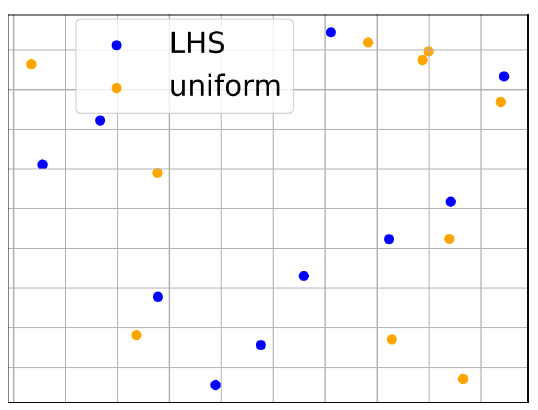
\includegraphics{../5-pictures/chapter-2_pic_2.png}
\caption{caption}
\end{figure}

    \begin{tcolorbox}[breakable, size=fbox, boxrule=1pt, pad at break*=1mm,colback=cellbackground, colframe=cellborder]
\prompt{In}{incolor}{156}{\boxspacing}
\begin{Verbatim}[commandchars=\\\{\}]
\PY{k+kn}{from} \PY{n+nn}{smt}\PY{n+nn}{.}\PY{n+nn}{sampling\PYZus{}methods} \PY{k+kn}{import} \PY{n}{LHS}
\end{Verbatim}
\end{tcolorbox}

    \begin{tcolorbox}[breakable, size=fbox, boxrule=1pt, pad at break*=1mm,colback=cellbackground, colframe=cellborder]
\prompt{In}{incolor}{157}{\boxspacing}
\begin{Verbatim}[commandchars=\\\{\}]
\PY{k}{def} \PY{n+nf}{lhs\PYZus{}sampling}\PY{p}{(}\PY{n}{rand}\PY{p}{,} \PY{n}{NUM}\PY{p}{,} \PY{n}{bounds}\PY{o}{=}\PY{k+kc}{None}\PY{p}{)}\PY{p}{:}

    \PY{n}{mInt} \PY{o}{=} \PY{p}{(}\PY{l+m+mi}{1} \PY{o}{\PYZlt{}\PYZlt{}} \PY{l+m+mi}{15}\PY{p}{)}
    \PY{n}{MInt} \PY{o}{=} \PY{p}{(}\PY{l+m+mi}{1} \PY{o}{\PYZlt{}\PYZlt{}} \PY{l+m+mi}{16}\PY{p}{)}
    \PY{n}{kw} \PY{o}{=} \PY{n+nb}{list}\PY{p}{(}\PY{n}{bounds}\PY{p}{)}

    \PY{c+c1}{\PYZsh{} builds the array of bounds}
    \PY{n}{limits} \PY{o}{=} \PY{n}{np}\PY{o}{.}\PY{n}{empty}\PY{p}{(} \PY{n}{shape}\PY{o}{=}\PY{p}{(}\PY{l+m+mi}{0}\PY{p}{,}\PY{l+m+mi}{2}\PY{p}{)} \PY{p}{)}
    \PY{k}{for} \PY{n}{k} \PY{o+ow}{in} \PY{n}{kw}\PY{p}{:} \PY{n}{limits} \PY{o}{=} \PY{n}{np}\PY{o}{.}\PY{n}{concatenate}\PY{p}{(}\PY{p}{(}\PY{n}{limits}\PY{p}{,} \PY{p}{[}\PY{n}{bounds}\PY{p}{[}\PY{n}{k}\PY{p}{]}\PY{p}{]}\PY{p}{)}\PY{p}{,} \PY{n}{axis}\PY{o}{=}\PY{l+m+mi}{0}\PY{p}{)}

    \PY{n}{sampling} \PY{o}{=} \PY{n}{LHS}\PY{p}{(}\PY{n}{xlimits}\PY{o}{=}\PY{n}{limits}\PY{p}{,} \PY{n}{random\PYZus{}state}\PY{o}{=}\PY{n}{rand}\PY{o}{.}\PY{n}{randint}\PY{p}{(}\PY{n}{mInt}\PY{p}{,}\PY{n}{MInt}\PY{p}{)}\PY{p}{)}
    \PY{n}{x}   \PY{o}{=} \PY{n}{sampling}\PY{p}{(}\PY{n}{NUM}\PY{p}{)}

    \PY{n}{X} \PY{o}{=} \PY{n}{pd}\PY{o}{.}\PY{n}{DataFrame}\PY{p}{(}\PY{p}{)}
    \PY{k}{for} \PY{n}{n} \PY{o+ow}{in} \PY{n+nb}{range}\PY{p}{(}\PY{n+nb}{len}\PY{p}{(}\PY{n}{kw}\PY{p}{)}\PY{p}{)}\PY{p}{:}
        \PY{n}{tag} \PY{o}{=} \PY{n}{kw}\PY{p}{[}\PY{n}{n}\PY{p}{]}
        \PY{n}{X}\PY{p}{[}\PY{n}{tag}\PY{p}{]} \PY{o}{=} \PY{n}{x}\PY{p}{[}\PY{p}{:}\PY{p}{,}\PY{n}{n}\PY{p}{]}

    \PY{k}{return} \PY{n}{X}
\end{Verbatim}
\end{tcolorbox}

    \hypertarget{sample-generator}{%
\subsubsection{Sample Generator}\label{sample-generator}}

    We assume $r = q = 0, S_0 = 1$ and create a data set of 1000000
observations by randomly sampling from uniform distributions for the
other five inputs to the Black-Scholes-Merton formula. The lower and
upper bounds of the uniform distributions are as indicated in the
\texttt{bounds} dictionary. For each set of parameters sampled, we
calculate the Black-Scholes-Merton price using equations \eqref{eq:1}
and \eqref{eq:2}.

    \begin{tcolorbox}[breakable, size=fbox, boxrule=1pt, pad at break*=1mm,colback=cellbackground, colframe=cellborder]
\prompt{In}{incolor}{201}{\boxspacing}
\begin{Verbatim}[commandchars=\\\{\}]
\PY{c+c1}{\PYZsh{} For the neural network calculating the vanilla option prices in the Black Scholes model, }
\PY{c+c1}{\PYZsh{} the features used are the time to maturity T, the moneyness (simply defined as \PYZsq{}Strike\PYZsq{}) }
\PY{c+c1}{\PYZsh{} and the asset volatility sigma.}
\PY{c+c1}{\PYZsh{}}
\PY{c+c1}{\PYZsh{} Lower and upper boundaries for each parameter}
\PY{c+c1}{\PYZsh{}}
\PY{n}{bounds} \PY{o}{=} \PY{p}{\PYZob{}}  \PY{l+s+s2}{\PYZdq{}}\PY{l+s+s2}{T}\PY{l+s+s2}{\PYZdq{}}     \PY{p}{:} \PY{p}{[}\PY{l+m+mf}{1.}\PY{o}{/}\PY{l+m+mf}{12.}\PY{p}{,} \PY{l+m+mf}{2.00}\PY{p}{]}
          \PY{p}{,} \PY{l+s+s2}{\PYZdq{}}\PY{l+s+s2}{Sigma}\PY{l+s+s2}{\PYZdq{}} \PY{p}{:} \PY{p}{[} \PY{o}{.}\PY{l+m+mi}{01}  \PY{p}{,}  \PY{o}{.}\PY{l+m+mi}{80}\PY{p}{]}
          \PY{p}{,} \PY{l+s+s2}{\PYZdq{}}\PY{l+s+s2}{Strike}\PY{l+s+s2}{\PYZdq{}}\PY{p}{:} \PY{p}{[} \PY{o}{.}\PY{l+m+mi}{4}   \PY{p}{,} \PY{l+m+mf}{1.20}\PY{p}{]}
         \PY{p}{\PYZcb{}}
\PY{c+c1}{\PYZsh{}}
\PY{c+c1}{\PYZsh{} Number of Observations}
\PY{c+c1}{\PYZsh{}}
\PY{n}{NUM} \PY{o}{=} \PY{l+m+mi}{100000}
\PY{c+c1}{\PYZsh{}}
\PY{c+c1}{\PYZsh{} Random number generator}
\PY{c+c1}{\PYZsh{}}
\PY{n}{seed} \PY{o}{=} \PY{l+m+mi}{42}
\PY{n}{rand} \PY{o}{=} \PY{n}{np}\PY{o}{.}\PY{n}{random}\PY{o}{.}\PY{n}{RandomState}\PY{p}{(}\PY{n}{seed}\PY{p}{)}
\PY{c+c1}{\PYZsh{}}
\PY{c+c1}{\PYZsh{} Latin Hypercube Sampling}
\PY{c+c1}{\PYZsh{}}
\PY{n}{xDF} \PY{o}{=} \PY{n}{lhs\PYZus{}sampling}\PY{p}{(}\PY{n}{rand}\PY{p}{,} \PY{n}{NUM}\PY{p}{,} \PY{n}{bounds}\PY{o}{=}\PY{n}{bounds}\PY{p}{)}
\PY{n}{xDF}\PY{o}{.}\PY{n}{head}\PY{p}{(}\PY{p}{)}
\end{Verbatim}
\end{tcolorbox}

            \begin{tcolorbox}[breakable, size=fbox, boxrule=.5pt, pad at break*=1mm, opacityfill=0]
\prompt{Out}{outcolor}{201}{\boxspacing}
\begin{Verbatim}[commandchars=\\\{\}]
          T     Sigma    Strike
0  1.994528  0.030157  1.006996
1  1.413241  0.423980  1.055836
2  0.891927  0.673083  0.677284
3  0.903523  0.308853  0.623468
4  1.298069  0.134919  0.743884
\end{Verbatim}
\end{tcolorbox}
        
    \begin{tcolorbox}[breakable, size=fbox, boxrule=1pt, pad at break*=1mm,colback=cellbackground, colframe=cellborder]
\prompt{In}{incolor}{202}{\boxspacing}
\begin{Verbatim}[commandchars=\\\{\}]
\PY{n}{xDF}\PY{o}{.}\PY{n}{hist}\PY{p}{(}\PY{p}{)}
\end{Verbatim}
\end{tcolorbox}

            \begin{tcolorbox}[breakable, size=fbox, boxrule=.5pt, pad at break*=1mm, opacityfill=0]
\prompt{Out}{outcolor}{202}{\boxspacing}
\begin{Verbatim}[commandchars=\\\{\}]
array([[<matplotlib.axes.\_subplots.AxesSubplot object at 0x000001DD418D0BC8>,
        <matplotlib.axes.\_subplots.AxesSubplot object at 0x000001DD41869888>],
       [<matplotlib.axes.\_subplots.AxesSubplot object at 0x000001DD397B0408>,
        <matplotlib.axes.\_subplots.AxesSubplot object at 0x000001DD397CA8C8>]],
      dtype=object)
\end{Verbatim}
\end{tcolorbox}
        
    \begin{center}
    \adjustimage{max size={0.9\linewidth}{0.9\paperheight}}{output_19_1.png}
    \end{center}
    { \hspace*{\fill} \\}
    
    \begin{tcolorbox}[breakable, size=fbox, boxrule=1pt, pad at break*=1mm,colback=cellbackground, colframe=cellborder]
\prompt{In}{incolor}{203}{\boxspacing}
\begin{Verbatim}[commandchars=\\\{\}]
\PY{k}{def} \PY{n+nf}{gen}\PY{p}{(}\PY{n}{NUM}\PY{p}{,} \PY{n}{lhs}\PY{p}{)}\PY{p}{:}

    \PY{l+s+sd}{\PYZsq{}\PYZsq{}\PYZsq{}}
\PY{l+s+sd}{    A NumPy optimized data generator}
\PY{l+s+sd}{    \PYZsq{}\PYZsq{}\PYZsq{}}
    \PY{n}{x}   \PY{o}{=} \PY{n}{lhs}

    \PY{n}{\PYZus{}\PYZus{}tStart} \PY{o}{=} \PY{n}{time}\PY{o}{.}\PY{n}{perf\PYZus{}counter}\PY{p}{(}\PY{p}{)}
    \PY{n}{S0}     \PY{o}{=} \PY{n}{np}\PY{o}{.}\PY{n}{full}\PY{p}{(}\PY{n}{NUM}\PY{p}{,} \PY{l+m+mf}{1.0}\PY{p}{,} \PY{n}{dtype} \PY{o}{=} \PY{n}{np}\PY{o}{.}\PY{n}{double}\PY{p}{)}
    \PY{n}{r}      \PY{o}{=} \PY{n}{np}\PY{o}{.}\PY{n}{full}\PY{p}{(}\PY{n}{NUM}\PY{p}{,} \PY{l+m+mf}{0.0}\PY{p}{,} \PY{n}{dtype} \PY{o}{=} \PY{n}{np}\PY{o}{.}\PY{n}{double}\PY{p}{)}
    \PY{n}{price}  \PY{o}{=} \PY{n}{np\PYZus{}euro\PYZus{}call}\PY{p}{(}\PY{n}{S0}\PY{p}{,} \PY{n}{r}\PY{p}{,} \PY{n}{x}\PY{p}{[}\PY{l+s+s2}{\PYZdq{}}\PY{l+s+s2}{T}\PY{l+s+s2}{\PYZdq{}}\PY{p}{]}\PY{p}{,} \PY{n}{x}\PY{p}{[}\PY{l+s+s2}{\PYZdq{}}\PY{l+s+s2}{Sigma}\PY{l+s+s2}{\PYZdq{}}\PY{p}{]}\PY{p}{,} \PY{n}{x}\PY{p}{[}\PY{l+s+s2}{\PYZdq{}}\PY{l+s+s2}{Strike}\PY{l+s+s2}{\PYZdq{}}\PY{p}{]}\PY{p}{)}
    \PY{n}{\PYZus{}\PYZus{}tEnd} \PY{o}{=} \PY{n}{time}\PY{o}{.}\PY{n}{perf\PYZus{}counter}\PY{p}{(}\PY{p}{)}
    \PY{n+nb}{print}\PY{p}{(}\PY{l+s+s2}{\PYZdq{}}\PY{l+s+s2}{@ }\PY{l+s+si}{\PYZpc{}\PYZhy{}34s}\PY{l+s+s2}{: elapsed }\PY{l+s+si}{\PYZpc{}.4f}\PY{l+s+s2}{ sec}\PY{l+s+s2}{\PYZdq{}} \PY{o}{\PYZpc{}}\PY{p}{(}\PY{l+s+s2}{\PYZdq{}}\PY{l+s+s2}{NP pricing}\PY{l+s+s2}{\PYZdq{}}\PY{p}{,} \PY{n}{\PYZus{}\PYZus{}tEnd}\PY{o}{\PYZhy{}}\PY{n}{\PYZus{}\PYZus{}tStart}\PY{p}{)} \PY{p}{)}

    \PY{n}{df} \PY{o}{=} \PY{n}{pd}\PY{o}{.}\PY{n}{DataFrame}\PY{p}{(}\PY{n}{x}\PY{p}{)}
    \PY{n}{df}\PY{p}{[}\PY{l+s+s2}{\PYZdq{}}\PY{l+s+s2}{Price}\PY{l+s+s2}{\PYZdq{}}\PY{p}{]} \PY{o}{=} \PY{n}{price}

    \PY{k}{return} \PY{n}{df}
\end{Verbatim}
\end{tcolorbox}

    \begin{tcolorbox}[breakable, size=fbox, boxrule=1pt, pad at break*=1mm,colback=cellbackground, colframe=cellborder]
\prompt{In}{incolor}{204}{\boxspacing}
\begin{Verbatim}[commandchars=\\\{\}]
\PY{n}{\PYZus{}\PYZus{}tStart} \PY{o}{=} \PY{n}{time}\PY{o}{.}\PY{n}{perf\PYZus{}counter}\PY{p}{(}\PY{p}{)}
\PY{n}{df} \PY{o}{=}  \PY{n}{gen}\PY{p}{(}\PY{n}{NUM}\PY{p}{,} \PY{n}{xDF}\PY{p}{)}
\PY{n}{\PYZus{}\PYZus{}tEnd} \PY{o}{=} \PY{n}{time}\PY{o}{.}\PY{n}{perf\PYZus{}counter}\PY{p}{(}\PY{p}{)}
\PY{n+nb}{print}\PY{p}{(}\PY{l+s+s2}{\PYZdq{}}\PY{l+s+s2}{@ }\PY{l+s+si}{\PYZpc{}\PYZhy{}34s}\PY{l+s+s2}{: elapsed }\PY{l+s+si}{\PYZpc{}.4f}\PY{l+s+s2}{ sec}\PY{l+s+s2}{\PYZdq{}} \PY{o}{\PYZpc{}}\PY{p}{(}\PY{l+s+s2}{\PYZdq{}}\PY{l+s+s2}{GEN}\PY{l+s+s2}{\PYZdq{}}\PY{p}{,} \PY{n}{\PYZus{}\PYZus{}tEnd} \PY{o}{\PYZhy{}} \PY{n}{\PYZus{}\PYZus{}tStart}\PY{p}{)} \PY{p}{)}

\PY{n}{df}\PY{o}{.}\PY{n}{head}\PY{p}{(}\PY{p}{)}
\end{Verbatim}
\end{tcolorbox}

    \begin{Verbatim}[commandchars=\\\{\}]
@ NP pricing                        : elapsed 0.0484 sec
@ GEN                               : elapsed 0.0501 sec
    \end{Verbatim}

            \begin{tcolorbox}[breakable, size=fbox, boxrule=.5pt, pad at break*=1mm, opacityfill=0]
\prompt{Out}{outcolor}{204}{\boxspacing}
\begin{Verbatim}[commandchars=\\\{\}]
          T     Sigma    Strike     Price
0  1.994528  0.030157  1.006996  0.013779
1  1.413241  0.423980  1.055836  0.177768
2  0.891927  0.673083  0.677284  0.406779
3  0.903523  0.308853  0.623468  0.381761
4  1.298069  0.134919  0.743884  0.257487
\end{Verbatim}
\end{tcolorbox}
        
    \begin{tcolorbox}[breakable, size=fbox, boxrule=1pt, pad at break*=1mm,colback=cellbackground, colframe=cellborder]
\prompt{In}{incolor}{205}{\boxspacing}
\begin{Verbatim}[commandchars=\\\{\}]
\PY{n}{X\PYZus{}train}\PY{p}{,} \PY{n}{X\PYZus{}test} \PY{o}{=} \PY{n}{train\PYZus{}test\PYZus{}split}\PY{p}{(}\PY{n}{df}\PY{p}{,} \PY{n}{test\PYZus{}size}\PY{o}{=}\PY{l+m+mf}{0.33}\PY{p}{,} \PY{n}{random\PYZus{}state}\PY{o}{=}\PY{l+m+mi}{42}\PY{p}{)}
\PY{n+nb}{print}\PY{p}{(}\PY{n+nb}{len}\PY{p}{(}\PY{n}{X\PYZus{}train}\PY{p}{)}\PY{p}{,} \PY{n+nb}{len}\PY{p}{(}\PY{n}{X\PYZus{}test}\PY{p}{)}\PY{p}{)}
\PY{n}{X\PYZus{}train}\PY{o}{.}\PY{n}{head}\PY{p}{(}\PY{p}{)}
\end{Verbatim}
\end{tcolorbox}

    \begin{Verbatim}[commandchars=\\\{\}]
67000 33000
    \end{Verbatim}

            \begin{tcolorbox}[breakable, size=fbox, boxrule=.5pt, pad at break*=1mm, opacityfill=0]
\prompt{Out}{outcolor}{205}{\boxspacing}
\begin{Verbatim}[commandchars=\\\{\}]
              T     Sigma    Strike     Price
59428  1.196045  0.739988  0.925964  0.340934
34957  1.703252  0.036864  1.071172  0.001712
4264   1.762209  0.204376  0.707052  0.303768
53791  1.717263  0.545387  0.556180  0.503275
82114  0.548441  0.620800  1.118916  0.138778
\end{Verbatim}
\end{tcolorbox}
        
    \begin{tcolorbox}[breakable, size=fbox, boxrule=1pt, pad at break*=1mm,colback=cellbackground, colframe=cellborder]
\prompt{In}{incolor}{206}{\boxspacing}
\begin{Verbatim}[commandchars=\\\{\}]
\PY{n}{X\PYZus{}test}\PY{o}{.}\PY{n}{head}\PY{p}{(}\PY{p}{)}
\end{Verbatim}
\end{tcolorbox}

            \begin{tcolorbox}[breakable, size=fbox, boxrule=.5pt, pad at break*=1mm, opacityfill=0]
\prompt{Out}{outcolor}{206}{\boxspacing}
\begin{Verbatim}[commandchars=\\\{\}]
              T     Sigma    Strike     Price
75721  0.117191  0.771398  1.086372  0.071709
80184  1.026228  0.200512  0.801388  0.211295
19864  0.342879  0.041699  0.713412  0.286588
76699  0.226135  0.336637  1.169668  0.014981
92991  0.936758  0.730681  1.048660  0.259367
\end{Verbatim}
\end{tcolorbox}
        
    To make the illustration more interesting, we then add a random error to
each calculated price. The random error is normally distributed with a
mean of zero and a standard deviation of
\(\epsilon \cdot (P_{max} - P_{min})\) where \(\epsilon\) is a scale
parameter defined by the user.

    \begin{tcolorbox}[breakable, size=fbox, boxrule=1pt, pad at break*=1mm,colback=cellbackground, colframe=cellborder]
\prompt{In}{incolor}{207}{\boxspacing}
\begin{Verbatim}[commandchars=\\\{\}]
\PY{k}{def} \PY{n+nf}{add\PYZus{}noise}\PY{p}{(}\PY{n}{rand}\PY{p}{,} \PY{n}{Xv}\PY{p}{,} \PY{n}{eps}\PY{p}{)}\PY{p}{:}
    \PY{n}{X}  \PY{o}{=} \PY{n}{Xv}\PY{o}{.}\PY{n}{copy}\PY{p}{(}\PY{p}{)}
    \PY{n}{xl} \PY{o}{=} \PY{n}{np}\PY{o}{.}\PY{n}{min}\PY{p}{(}\PY{n}{X}\PY{p}{[}\PY{l+s+s2}{\PYZdq{}}\PY{l+s+s2}{Price}\PY{l+s+s2}{\PYZdq{}}\PY{p}{]}\PY{p}{)}
    \PY{n}{xh} \PY{o}{=} \PY{n}{np}\PY{o}{.}\PY{n}{max}\PY{p}{(}\PY{n}{X}\PY{p}{[}\PY{l+s+s2}{\PYZdq{}}\PY{l+s+s2}{Price}\PY{l+s+s2}{\PYZdq{}}\PY{p}{]}\PY{p}{)}

    \PY{n}{xi} \PY{o}{=} \PY{n}{rand}\PY{o}{.}\PY{n}{normal}\PY{p}{(} \PY{n}{loc} \PY{o}{=} \PY{l+m+mf}{0.0}\PY{p}{,} \PY{n}{scale} \PY{o}{=} \PY{n}{eps}\PY{o}{*}\PY{p}{(}\PY{n}{xh}\PY{o}{\PYZhy{}}\PY{n}{xl}\PY{p}{)}\PY{p}{,} \PY{n}{size}\PY{o}{=}\PY{n}{X}\PY{o}{.}\PY{n}{shape}\PY{p}{[}\PY{l+m+mi}{0}\PY{p}{]}\PY{p}{)}
    \PY{n}{X}\PY{p}{[}\PY{l+s+s2}{\PYZdq{}}\PY{l+s+s2}{Price}\PY{l+s+s2}{\PYZdq{}}\PY{p}{]} \PY{o}{+}\PY{o}{=} \PY{n}{xi}
    \PY{k}{return} \PY{n}{X}
\end{Verbatim}
\end{tcolorbox}

    \begin{tcolorbox}[breakable, size=fbox, boxrule=1pt, pad at break*=1mm,colback=cellbackground, colframe=cellborder]
\prompt{In}{incolor}{208}{\boxspacing}
\begin{Verbatim}[commandchars=\\\{\}]
\PY{n}{EPS} \PY{o}{=} \PY{l+m+mf}{0.0}
\PY{k}{if} \PY{n}{EPS} \PY{o}{\PYZgt{}} \PY{l+m+mf}{0.0}\PY{p}{:} 
    \PY{n}{X\PYZus{}train} \PY{o}{=} \PY{n}{add\PYZus{}noise}\PY{p}{(}\PY{n}{rand}\PY{p}{,} \PY{n}{X\PYZus{}train}\PY{p}{,} \PY{n}{EPS}\PY{p}{)}
\end{Verbatim}
\end{tcolorbox}

    \begin{tcolorbox}[breakable, size=fbox, boxrule=1pt, pad at break*=1mm,colback=cellbackground, colframe=cellborder]
\prompt{In}{incolor}{209}{\boxspacing}
\begin{Verbatim}[commandchars=\\\{\}]
\PY{n}{y\PYZus{}train} \PY{o}{=} \PY{n}{X\PYZus{}train}\PY{p}{[}\PY{l+s+s1}{\PYZsq{}}\PY{l+s+s1}{Price}\PY{l+s+s1}{\PYZsq{}}\PY{p}{]}
\PY{n}{y\PYZus{}test}  \PY{o}{=} \PY{n}{X\PYZus{}test}\PY{p}{[}\PY{l+s+s1}{\PYZsq{}}\PY{l+s+s1}{Price}\PY{l+s+s1}{\PYZsq{}}\PY{p}{]}
\end{Verbatim}
\end{tcolorbox}

    \begin{tcolorbox}[breakable, size=fbox, boxrule=1pt, pad at break*=1mm,colback=cellbackground, colframe=cellborder]
\prompt{In}{incolor}{210}{\boxspacing}
\begin{Verbatim}[commandchars=\\\{\}]
\PY{n}{ax}\PY{o}{=}\PY{n}{y\PYZus{}train}\PY{o}{.}\PY{n}{plot}\PY{p}{(}\PY{n}{kind}\PY{o}{=}\PY{l+s+s1}{\PYZsq{}}\PY{l+s+s1}{hist}\PY{l+s+s1}{\PYZsq{}}\PY{p}{,} \PY{n}{bins}\PY{o}{=}\PY{l+m+mi}{100}\PY{p}{,} \PY{n}{grid}\PY{o}{=}\PY{k+kc}{False}\PY{p}{,} \PY{n}{figsize}\PY{o}{=}\PY{p}{(}\PY{l+m+mi}{12}\PY{p}{,}\PY{l+m+mi}{5}\PY{p}{)}\PY{p}{,} \PY{n}{color}\PY{o}{=}\PY{l+s+s1}{\PYZsq{}}\PY{l+s+s1}{green}\PY{l+s+s1}{\PYZsq{}}\PY{p}{,} \PY{n}{title} \PY{o}{=} \PY{l+s+s1}{\PYZsq{}}\PY{l+s+s1}{Training Set}\PY{l+s+s1}{\PYZsq{}}\PY{p}{)}
\PY{n}{ax}\PY{o}{.}\PY{n}{set\PYZus{}xlabel}\PY{p}{(}\PY{l+s+s1}{\PYZsq{}}\PY{l+s+s1}{BS Price}\PY{l+s+s1}{\PYZsq{}}\PY{p}{)}
\end{Verbatim}
\end{tcolorbox}

            \begin{tcolorbox}[breakable, size=fbox, boxrule=.5pt, pad at break*=1mm, opacityfill=0]
\prompt{Out}{outcolor}{210}{\boxspacing}
\begin{Verbatim}[commandchars=\\\{\}]
Text(0.5, 0, 'BS Price')
\end{Verbatim}
\end{tcolorbox}
        
    \begin{center}
    \adjustimage{max size={0.9\linewidth}{0.9\paperheight}}{output_28_1.png}
    \end{center}
    { \hspace*{\fill} \\}
    
    \begin{tcolorbox}[breakable, size=fbox, boxrule=1pt, pad at break*=1mm,colback=cellbackground, colframe=cellborder]
\prompt{In}{incolor}{211}{\boxspacing}
\begin{Verbatim}[commandchars=\\\{\}]
\PY{n}{ax}\PY{o}{=}\PY{n}{y\PYZus{}train}\PY{o}{.}\PY{n}{plot}\PY{p}{(}\PY{n}{kind}\PY{o}{=}\PY{l+s+s1}{\PYZsq{}}\PY{l+s+s1}{hist}\PY{l+s+s1}{\PYZsq{}}\PY{p}{,} \PY{n}{bins}\PY{o}{=}\PY{l+m+mi}{100}\PY{p}{,} \PY{n}{grid}\PY{o}{=}\PY{k+kc}{False}\PY{p}{,} \PY{n}{figsize}\PY{o}{=}\PY{p}{(}\PY{l+m+mi}{12}\PY{p}{,}\PY{l+m+mi}{5}\PY{p}{)}\PY{p}{,} \PY{n}{color}\PY{o}{=}\PY{l+s+s1}{\PYZsq{}}\PY{l+s+s1}{blue}\PY{l+s+s1}{\PYZsq{}}\PY{p}{,} \PY{n}{title} \PY{o}{=} \PY{l+s+s1}{\PYZsq{}}\PY{l+s+s1}{Test Set}\PY{l+s+s1}{\PYZsq{}}\PY{p}{)}
\PY{n}{ax}\PY{o}{.}\PY{n}{set\PYZus{}xlabel}\PY{p}{(}\PY{l+s+s1}{\PYZsq{}}\PY{l+s+s1}{BS Price}\PY{l+s+s1}{\PYZsq{}}\PY{p}{)}
\end{Verbatim}
\end{tcolorbox}

            \begin{tcolorbox}[breakable, size=fbox, boxrule=.5pt, pad at break*=1mm, opacityfill=0]
\prompt{Out}{outcolor}{211}{\boxspacing}
\begin{Verbatim}[commandchars=\\\{\}]
Text(0.5, 0, 'BS Price')
\end{Verbatim}
\end{tcolorbox}
        
    \begin{center}
    \adjustimage{max size={0.9\linewidth}{0.9\paperheight}}{output_29_1.png}
    \end{center}
    { \hspace*{\fill} \\}
    
    \begin{tcolorbox}[breakable, size=fbox, boxrule=1pt, pad at break*=1mm,colback=cellbackground, colframe=cellborder]
\prompt{In}{incolor}{212}{\boxspacing}
\begin{Verbatim}[commandchars=\\\{\}]
\PY{n}{X\PYZus{}train} \PY{o}{=} \PY{n}{X\PYZus{}train}\PY{o}{.}\PY{n}{drop}\PY{p}{(}\PY{p}{[}\PY{l+s+s1}{\PYZsq{}}\PY{l+s+s1}{Price}\PY{l+s+s1}{\PYZsq{}}\PY{p}{]}\PY{p}{,} \PY{n}{axis}\PY{o}{=}\PY{l+m+mi}{1}\PY{p}{)}
\PY{n}{X\PYZus{}test}  \PY{o}{=} \PY{n}{X\PYZus{}test}\PY{o}{.}\PY{n}{drop}\PY{p}{(}\PY{p}{[}\PY{l+s+s1}{\PYZsq{}}\PY{l+s+s1}{Price}\PY{l+s+s1}{\PYZsq{}}\PY{p}{]}\PY{p}{,} \PY{n}{axis}\PY{o}{=}\PY{l+m+mi}{1}\PY{p}{)}
\PY{n}{X\PYZus{}train}\PY{o}{.}\PY{n}{head}\PY{p}{(}\PY{p}{)}
\end{Verbatim}
\end{tcolorbox}

            \begin{tcolorbox}[breakable, size=fbox, boxrule=.5pt, pad at break*=1mm, opacityfill=0]
\prompt{Out}{outcolor}{212}{\boxspacing}
\begin{Verbatim}[commandchars=\\\{\}]
              T     Sigma    Strike
59428  1.196045  0.739988  0.925964
34957  1.703252  0.036864  1.071172
4264   1.762209  0.204376  0.707052
53791  1.717263  0.545387  0.556180
82114  0.548441  0.620800  1.118916
\end{Verbatim}
\end{tcolorbox}
        
    \hypertarget{scaling-data}{%
\subsubsection{Scaling Data}\label{scaling-data}}

    \begin{tcolorbox}[breakable, size=fbox, boxrule=1pt, pad at break*=1mm,colback=cellbackground, colframe=cellborder]
\prompt{In}{incolor}{213}{\boxspacing}
\begin{Verbatim}[commandchars=\\\{\}]
\PY{k+kn}{from} \PY{n+nn}{sklearn}\PY{n+nn}{.}\PY{n+nn}{preprocessing} \PY{k+kn}{import} \PY{n}{StandardScaler}

\PY{n}{scaling} \PY{o}{=} \PY{k+kc}{True}

\PY{k}{if} \PY{n}{scaling}\PY{p}{:}
    \PY{c+c1}{\PYZsh{} Scale the train set}
    \PY{n}{scaler} \PY{o}{=} \PY{n}{StandardScaler}\PY{p}{(}\PY{p}{)}\PY{o}{.}\PY{n}{fit}\PY{p}{(}\PY{n}{X\PYZus{}train}\PY{p}{)}
    \PY{n}{X\PYZus{}train} \PY{o}{=} \PY{n}{scaler}\PY{o}{.}\PY{n}{transform}\PY{p}{(}\PY{n}{X\PYZus{}train}\PY{p}{)}

    \PY{c+c1}{\PYZsh{} Scale the test set}
    \PY{n}{scaler} \PY{o}{=} \PY{n}{StandardScaler}\PY{p}{(}\PY{p}{)}\PY{o}{.}\PY{n}{fit}\PY{p}{(}\PY{n}{X\PYZus{}test}\PY{p}{)}
    \PY{n}{X\PYZus{}test} \PY{o}{=} \PY{n}{scaler}\PY{o}{.}\PY{n}{transform}\PY{p}{(}\PY{n}{X\PYZus{}test}\PY{p}{)}
    
    \PY{c+c1}{\PYZsh{} Transform into pd DataFrame}
    \PY{n}{X\PYZus{}train} \PY{o}{=} \PY{n}{pd}\PY{o}{.}\PY{n}{DataFrame}\PY{p}{(}\PY{n}{X\PYZus{}train}\PY{p}{)}
    \PY{n}{X\PYZus{}test} \PY{o}{=} \PY{n}{pd}\PY{o}{.}\PY{n}{DataFrame}\PY{p}{(}\PY{n}{X\PYZus{}test}\PY{p}{)}
\end{Verbatim}
\end{tcolorbox}

    \hypertarget{create-the-model}{%
\subsection{Create the Model}\label{create-the-model}}

    \hypertarget{neural-network-architecture}{%
\subsubsection{Neural Network
Architecture}\label{neural-network-architecture}}

    We use mean absolute error (mae) as the cost function. The neural
network has two hidden layers and a decreasing number of neurons per
layer. The relu activation function is used.

    \begin{tcolorbox}[breakable, size=fbox, boxrule=1pt, pad at break*=1mm,colback=cellbackground, colframe=cellborder]
\prompt{In}{incolor}{214}{\boxspacing}
\begin{Verbatim}[commandchars=\\\{\}]
\PY{k+kn}{from} \PY{n+nn}{keras}\PY{n+nn}{.}\PY{n+nn}{models} \PY{k+kn}{import} \PY{n}{Sequential}
\PY{k+kn}{from} \PY{n+nn}{keras}\PY{n+nn}{.}\PY{n+nn}{layers} \PY{k+kn}{import} \PY{n}{Dense}
\end{Verbatim}
\end{tcolorbox}

    \textbf{The input shape}

What flows between layers are tensors. Tensors can be seen as matrices,
with shapes. Shapes are consequences of the model's configuration.
Shapes are tuples representing how many elements an array or tensor has
in each dimension.

\begin{quote}
Ex: a shape (30,4,10) means an array or tensor with 3 dimensions,
containing 30 elements in the first dimension, 4 in the second and 10 in
the third, totaling 30\emph{4}10 = 1200 elements or numbers.
\end{quote}

In Keras, the input layer itself is not a layer, but a tensor. It's the
starting tensor you send to the first hidden layer. This tensor must
have the same shape as your training data.

\begin{quote}
Ex: if you have 30 images of 50x50 pixels in RGB (3 channels), the shape
of your input data is (30,50,50,3). Then your input layer tensor, must
have this shape.
\end{quote}

Since the input shape is the only one you need to define, Keras will
demand it in the first layer.

    \begin{tcolorbox}[breakable, size=fbox, boxrule=1pt, pad at break*=1mm,colback=cellbackground, colframe=cellborder]
\prompt{In}{incolor}{215}{\boxspacing}
\begin{Verbatim}[commandchars=\\\{\}]
\PY{k}{def} \PY{n+nf}{model\PYZus{}builder}\PY{p}{(} \PY{n}{inputShape} \PY{o}{=} \PY{p}{(}\PY{l+m+mi}{1}\PY{p}{,}\PY{p}{)}\PY{p}{)}\PY{p}{:}
    
    \PY{c+c1}{\PYZsh{} Initialize the constructor}
    \PY{n}{model} \PY{o}{=} \PY{n}{Sequential}\PY{p}{(}\PY{p}{)}

    \PY{c+c1}{\PYZsh{} Start from the first hidden layer, since the input is not actually a layer   }
    \PY{c+c1}{\PYZsh{} But inform the shape of the input, with inputShape elements.    }
    \PY{n}{model}\PY{o}{.}\PY{n}{add}\PY{p}{(}\PY{n}{Dense}\PY{p}{(}\PY{l+m+mi}{200}\PY{p}{,} \PY{n}{activation}\PY{o}{=}\PY{l+s+s1}{\PYZsq{}}\PY{l+s+s1}{relu}\PY{l+s+s1}{\PYZsq{}}\PY{p}{,} \PY{n}{input\PYZus{}shape}\PY{o}{=}\PY{n}{inputShape}\PY{p}{)}\PY{p}{)}

    \PY{c+c1}{\PYZsh{} Add one more hidden layer }
    \PY{n}{model}\PY{o}{.}\PY{n}{add}\PY{p}{(}\PY{n}{Dense}\PY{p}{(}\PY{l+m+mi}{200}\PY{p}{,} \PY{n}{activation}\PY{o}{=}\PY{l+s+s1}{\PYZsq{}}\PY{l+s+s1}{relu}\PY{l+s+s1}{\PYZsq{}}\PY{p}{)}\PY{p}{)}

    \PY{c+c1}{\PYZsh{} Add one more hidden layer }
    \PY{n}{model}\PY{o}{.}\PY{n}{add}\PY{p}{(}\PY{n}{Dense}\PY{p}{(}\PY{l+m+mi}{200}\PY{p}{,} \PY{n}{activation}\PY{o}{=}\PY{l+s+s1}{\PYZsq{}}\PY{l+s+s1}{relu}\PY{l+s+s1}{\PYZsq{}}\PY{p}{)}\PY{p}{)}

    \PY{c+c1}{\PYZsh{} Add an output layer }
    \PY{n}{model}\PY{o}{.}\PY{n}{add}\PY{p}{(}\PY{n}{Dense}\PY{p}{(}\PY{l+m+mi}{1}\PY{p}{)}\PY{p}{)}
    \PY{c+c1}{\PYZsh{} End model construction}

    \PY{c+c1}{\PYZsh{} Model output shape}
    \PY{n+nb}{print}\PY{p}{(}\PY{l+s+s2}{\PYZdq{}}\PY{l+s+s2}{model.output\PYZus{}shape: }\PY{l+s+si}{\PYZpc{}s}\PY{l+s+s2}{\PYZdq{}} \PY{o}{\PYZpc{}}\PY{p}{(}\PY{n+nb}{str}\PY{p}{(}\PY{n}{model}\PY{o}{.}\PY{n}{output\PYZus{}shape}\PY{p}{)}\PY{p}{)}\PY{p}{)}

    \PY{c+c1}{\PYZsh{} Model summary}
    \PY{n+nb}{print}\PY{p}{(}\PY{l+s+s2}{\PYZdq{}}\PY{l+s+s2}{Model.summary}\PY{l+s+s2}{\PYZdq{}}\PY{p}{)}\PY{p}{;} \PY{n}{model}\PY{o}{.}\PY{n}{summary}\PY{p}{(}\PY{p}{)}

    \PY{c+c1}{\PYZsh{} Model config}
    \PY{n+nb}{print}\PY{p}{(}\PY{l+s+s2}{\PYZdq{}}\PY{l+s+s2}{Model.config}\PY{l+s+s2}{\PYZdq{}}\PY{p}{)}\PY{p}{;} \PY{n}{model}\PY{o}{.}\PY{n}{get\PYZus{}config}\PY{p}{(}\PY{p}{)}

    \PY{n}{model}\PY{o}{.}\PY{n}{compile}\PY{p}{(}\PY{n}{loss}\PY{o}{=}\PY{l+s+s1}{\PYZsq{}}\PY{l+s+s1}{mse}\PY{l+s+s1}{\PYZsq{}}\PY{p}{,} \PY{n}{optimizer}\PY{o}{=}\PY{l+s+s1}{\PYZsq{}}\PY{l+s+s1}{rmsprop}\PY{l+s+s1}{\PYZsq{}}\PY{p}{,} \PY{n}{metrics}\PY{o}{=}\PY{p}{[}\PY{l+s+s1}{\PYZsq{}}\PY{l+s+s1}{mae}\PY{l+s+s1}{\PYZsq{}}\PY{p}{]}\PY{p}{)}
    \PY{k}{return} \PY{n}{model}
\end{Verbatim}
\end{tcolorbox}

    \begin{tcolorbox}[breakable, size=fbox, boxrule=1pt, pad at break*=1mm,colback=cellbackground, colframe=cellborder]
\prompt{In}{incolor}{216}{\boxspacing}
\begin{Verbatim}[commandchars=\\\{\}]
\PY{n}{model} \PY{o}{=} \PY{n}{model\PYZus{}builder}\PY{p}{(} \PY{n}{inputShape} \PY{o}{=} \PY{p}{(}\PY{n}{X\PYZus{}train}\PY{o}{.}\PY{n}{shape}\PY{p}{[}\PY{l+m+mi}{1}\PY{p}{]}\PY{p}{,}\PY{p}{)}\PY{p}{)}
\end{Verbatim}
\end{tcolorbox}

    \begin{Verbatim}[commandchars=\\\{\}]
model.output\_shape: (None, 1)
Model.summary
Model: "sequential\_7"
\_\_\_\_\_\_\_\_\_\_\_\_\_\_\_\_\_\_\_\_\_\_\_\_\_\_\_\_\_\_\_\_\_\_\_\_\_\_\_\_\_\_\_\_\_\_\_\_\_\_\_\_\_\_\_\_\_\_\_\_\_\_\_\_\_
Layer (type)                 Output Shape              Param \#
=================================================================
dense\_28 (Dense)             (None, 200)               800
\_\_\_\_\_\_\_\_\_\_\_\_\_\_\_\_\_\_\_\_\_\_\_\_\_\_\_\_\_\_\_\_\_\_\_\_\_\_\_\_\_\_\_\_\_\_\_\_\_\_\_\_\_\_\_\_\_\_\_\_\_\_\_\_\_
dense\_29 (Dense)             (None, 200)               40200
\_\_\_\_\_\_\_\_\_\_\_\_\_\_\_\_\_\_\_\_\_\_\_\_\_\_\_\_\_\_\_\_\_\_\_\_\_\_\_\_\_\_\_\_\_\_\_\_\_\_\_\_\_\_\_\_\_\_\_\_\_\_\_\_\_
dense\_30 (Dense)             (None, 200)               40200
\_\_\_\_\_\_\_\_\_\_\_\_\_\_\_\_\_\_\_\_\_\_\_\_\_\_\_\_\_\_\_\_\_\_\_\_\_\_\_\_\_\_\_\_\_\_\_\_\_\_\_\_\_\_\_\_\_\_\_\_\_\_\_\_\_
dense\_31 (Dense)             (None, 1)                 201
=================================================================
Total params: 81,401
Trainable params: 81,401
Non-trainable params: 0
\_\_\_\_\_\_\_\_\_\_\_\_\_\_\_\_\_\_\_\_\_\_\_\_\_\_\_\_\_\_\_\_\_\_\_\_\_\_\_\_\_\_\_\_\_\_\_\_\_\_\_\_\_\_\_\_\_\_\_\_\_\_\_\_\_
Model.config
    \end{Verbatim}

    \hypertarget{train-the-model}{%
\subsection{Train the Model}\label{train-the-model}}

    \begin{tcolorbox}[breakable, size=fbox, boxrule=1pt, pad at break*=1mm,colback=cellbackground, colframe=cellborder]
\prompt{In}{incolor}{217}{\boxspacing}
\begin{Verbatim}[commandchars=\\\{\}]
\PY{k}{def} \PY{n+nf}{show\PYZus{}scattered}\PY{p}{(} \PY{n}{y}\PY{p}{,} \PY{n}{t}\PY{p}{,} \PY{n}{TAG}\PY{p}{,} \PY{n}{ax} \PY{o}{=} \PY{k+kc}{None}\PY{p}{)}\PY{p}{:}
    \PY{c+c1}{\PYZsh{}x      = model.predict(X)}
    \PY{c+c1}{\PYZsh{}y      = np.ravel(x)}
    \PY{n}{xMin} \PY{o}{=} \PY{n+nb}{min}\PY{p}{(}\PY{n}{t}\PY{p}{)}
    \PY{n}{xMax} \PY{o}{=} \PY{n+nb}{max}\PY{p}{(}\PY{n}{t}\PY{p}{)}
    \PY{n}{v}    \PY{o}{=} \PY{n}{np}\PY{o}{.}\PY{n}{arange}\PY{p}{(}\PY{n}{xMin}\PY{p}{,} \PY{n}{xMax}\PY{p}{,} \PY{p}{(}\PY{n}{xMax}\PY{o}{\PYZhy{}}\PY{n}{xMin}\PY{p}{)}\PY{o}{/}\PY{l+m+mf}{100.}\PY{p}{)}

    \PY{n}{diff}   \PY{o}{=} \PY{n}{np}\PY{o}{.}\PY{n}{fabs}\PY{p}{(}\PY{n}{y} \PY{o}{\PYZhy{}} \PY{n}{t}\PY{p}{)}
    \PY{n+nb}{print}\PY{p}{(}\PY{l+s+s2}{\PYZdq{}}\PY{l+s+s2}{@ }\PY{l+s+si}{\PYZpc{}\PYZhy{}24s}\PY{l+s+s2}{: E[y\PYZhy{}t]: }\PY{l+s+si}{\PYZpc{}.6f}\PY{l+s+s2}{ Std(y\PYZhy{}t): }\PY{l+s+si}{\PYZpc{}.6f}\PY{l+s+s2}{\PYZdq{}} \PY{o}{\PYZpc{}}\PY{p}{(} \PY{n}{TAG}\PY{p}{,} \PY{n}{np}\PY{o}{.}\PY{n}{mean}\PY{p}{(}\PY{n}{diff}\PY{p}{)}\PY{p}{,} \PY{n}{np}\PY{o}{.}\PY{n}{std}\PY{p}{(}\PY{n}{diff}\PY{p}{)}\PY{p}{)}\PY{p}{)}
    \PY{k}{if} \PY{n}{ax} \PY{o}{==} \PY{k+kc}{None}\PY{p}{:} \PY{k}{return}

    \PY{n}{ax}\PY{o}{.}\PY{n}{plot}\PY{p}{(} \PY{n}{y}\PY{p}{,} \PY{n}{t}\PY{p}{,} \PY{l+s+s2}{\PYZdq{}}\PY{l+s+s2}{.}\PY{l+s+s2}{\PYZdq{}}\PY{p}{)}
    \PY{n}{ax}\PY{o}{.}\PY{n}{plot}\PY{p}{(} \PY{n}{v}\PY{p}{,} \PY{n}{v}\PY{p}{,} \PY{n}{color}\PY{o}{=}\PY{l+s+s2}{\PYZdq{}}\PY{l+s+s2}{red}\PY{l+s+s2}{\PYZdq{}}\PY{p}{)}
    \PY{n}{ax}\PY{o}{.}\PY{n}{set\PYZus{}title}\PY{p}{(}\PY{l+s+s2}{\PYZdq{}}\PY{l+s+si}{\PYZpc{}s}\PY{l+s+s2}{ mae=}\PY{l+s+si}{\PYZpc{}8.4f}\PY{l+s+s2}{, std=}\PY{l+s+si}{\PYZpc{}8.4f}\PY{l+s+s2}{\PYZdq{}} \PY{o}{\PYZpc{}}\PY{p}{(}\PY{n}{TAG}\PY{p}{,} \PY{n}{np}\PY{o}{.}\PY{n}{mean}\PY{p}{(}\PY{n}{diff}\PY{p}{)}\PY{p}{,} \PY{n}{np}\PY{o}{.}\PY{n}{std}\PY{p}{(}\PY{n}{diff}\PY{p}{)}\PY{p}{)}\PY{p}{)}
    \PY{n}{ax}\PY{o}{.}\PY{n}{set\PYZus{}xlabel}\PY{p}{(}\PY{l+s+s2}{\PYZdq{}}\PY{l+s+s2}{predicted}\PY{l+s+s2}{\PYZdq{}}\PY{p}{)}
    \PY{n}{ax}\PY{o}{.}\PY{n}{set\PYZus{}ylabel}\PY{p}{(}\PY{l+s+s2}{\PYZdq{}}\PY{l+s+s2}{target}\PY{l+s+s2}{\PYZdq{}}\PY{p}{)}
\end{Verbatim}
\end{tcolorbox}

    \begin{tcolorbox}[breakable, size=fbox, boxrule=1pt, pad at break*=1mm,colback=cellbackground, colframe=cellborder]
\prompt{In}{incolor}{218}{\boxspacing}
\begin{Verbatim}[commandchars=\\\{\}]
\PY{k}{def} \PY{n+nf}{display\PYZus{}nn\PYZus{}results}\PY{p}{(} \PY{n}{model}\PY{p}{,} \PY{n}{X\PYZus{}train}\PY{p}{,} \PY{n}{X\PYZus{}test}\PY{p}{,} \PY{n}{t\PYZus{}train}\PY{p}{,} \PY{n}{t\PYZus{}test}\PY{p}{,} \PY{n}{resFile}\PY{o}{=}\PY{k+kc}{None}\PY{p}{)}\PY{p}{:}

    \PY{n}{fig}\PY{p}{,} \PY{n}{ax} \PY{o}{=} \PY{n}{plt}\PY{o}{.}\PY{n}{subplots}\PY{p}{(}\PY{l+m+mi}{1}\PY{p}{,}\PY{l+m+mi}{2}\PY{p}{,} \PY{n}{figsize}\PY{o}{=}\PY{p}{(}\PY{l+m+mi}{12}\PY{p}{,}\PY{l+m+mi}{6}\PY{p}{)}\PY{p}{)}
    \PY{n}{fig}\PY{o}{.}\PY{n}{suptitle}\PY{p}{(}\PY{l+s+s2}{\PYZdq{}}\PY{l+s+s2}{Scattered plots}\PY{l+s+s2}{\PYZdq{}}\PY{p}{)}
    \PY{c+c1}{\PYZsh{}}
    \PY{c+c1}{\PYZsh{} The numpy module ravel of NumPy provides a function, called numpy.ravel, which is used to change }
    \PY{c+c1}{\PYZsh{} a 2\PYZhy{}dimensional array or a multi\PYZhy{}dimensional array into a contiguous flattened array. The returned }
    \PY{c+c1}{\PYZsh{} array has the same data type as the source array or input array.}
    \PY{c+c1}{\PYZsh{}}
    \PY{n}{y\PYZus{}train}  \PY{o}{=} \PY{n}{np}\PY{o}{.}\PY{n}{ravel}\PY{p}{(}\PY{n}{model}\PY{o}{.}\PY{n}{predict}\PY{p}{(}\PY{n}{X\PYZus{}train}\PY{p}{)}\PY{p}{)}
    \PY{n}{show\PYZus{}scattered}\PY{p}{(} \PY{n}{y\PYZus{}train}\PY{p}{,} \PY{n}{t\PYZus{}train}\PY{p}{,} \PY{l+s+s2}{\PYZdq{}}\PY{l+s+s2}{InSample}\PY{l+s+s2}{\PYZdq{}}\PY{p}{,} \PY{n}{ax} \PY{o}{=} \PY{n}{ax}\PY{p}{[}\PY{l+m+mi}{0}\PY{p}{]}\PY{p}{)}
    \PY{n}{diff}   \PY{o}{=} \PY{n}{np}\PY{o}{.}\PY{n}{fabs}\PY{p}{(}\PY{n}{y\PYZus{}train} \PY{o}{\PYZhy{}} \PY{n}{t\PYZus{}train}\PY{p}{)}
    \PY{n}{delta}  \PY{o}{=} \PY{n}{y\PYZus{}train} \PY{o}{\PYZhy{}} \PY{n}{t\PYZus{}train}
    \PY{n}{RES}    \PY{o}{=} \PY{n}{pd}\PY{o}{.}\PY{n}{DataFrame}\PY{p}{(}\PY{p}{\PYZob{}}\PY{l+s+s2}{\PYZdq{}}\PY{l+s+s2}{predicted}\PY{l+s+s2}{\PYZdq{}}\PY{p}{:} \PY{n}{y\PYZus{}train}\PY{p}{,} \PY{l+s+s2}{\PYZdq{}}\PY{l+s+s2}{target}\PY{l+s+s2}{\PYZdq{}}\PY{p}{:} \PY{n}{t\PYZus{}train}\PY{p}{,} \PY{l+s+s2}{\PYZdq{}}\PY{l+s+s2}{err}\PY{l+s+s2}{\PYZdq{}}\PY{p}{:} \PY{n}{diff}\PY{p}{,} \PY{l+s+s2}{\PYZdq{}}\PY{l+s+s2}{delta}\PY{l+s+s2}{\PYZdq{}}\PY{p}{:} \PY{n}{delta}\PY{p}{\PYZcb{}}\PY{p}{)}
    \PY{n}{h1}     \PY{o}{=} \PY{n}{RES}\PY{p}{[}\PY{l+s+s1}{\PYZsq{}}\PY{l+s+s1}{delta}\PY{l+s+s1}{\PYZsq{}}\PY{p}{]} 
    \PY{n}{RES}\PY{o}{.}\PY{n}{to\PYZus{}csv}\PY{p}{(}\PY{l+s+s2}{\PYZdq{}}\PY{l+s+s2}{res\PYZus{}in\PYZus{}sample.csv}\PY{l+s+s2}{\PYZdq{}}\PY{p}{,} \PY{n}{sep}\PY{o}{=}\PY{l+s+s1}{\PYZsq{}}\PY{l+s+s1}{,}\PY{l+s+s1}{\PYZsq{}}\PY{p}{,} \PY{n}{float\PYZus{}format}\PY{o}{=}\PY{l+s+s2}{\PYZdq{}}\PY{l+s+si}{\PYZpc{}.6f}\PY{l+s+s2}{\PYZdq{}}\PY{p}{,} \PY{n}{index}\PY{o}{=}\PY{k+kc}{True}\PY{p}{)}
    \PY{n+nb}{print}\PY{p}{(}\PY{l+s+s2}{\PYZdq{}}\PY{l+s+s2}{@}\PY{l+s+s2}{\PYZdq{}}\PY{p}{)}
    
    \PY{n}{y\PYZus{}test}  \PY{o}{=} \PY{n}{np}\PY{o}{.}\PY{n}{ravel}\PY{p}{(}\PY{n}{model}\PY{o}{.}\PY{n}{predict}\PY{p}{(}\PY{n}{X\PYZus{}test}\PY{p}{)}\PY{p}{)}
    \PY{n}{show\PYZus{}scattered}\PY{p}{(} \PY{n}{y\PYZus{}test} \PY{p}{,} \PY{n}{t\PYZus{}test}\PY{p}{,} \PY{l+s+s2}{\PYZdq{}}\PY{l+s+s2}{OutOfSample}\PY{l+s+s2}{\PYZdq{}}\PY{p}{,} \PY{n}{ax}\PY{o}{=} \PY{n}{ax}\PY{p}{[}\PY{l+m+mi}{1}\PY{p}{]}\PY{p}{)}
    \PY{n}{diff}   \PY{o}{=} \PY{n}{np}\PY{o}{.}\PY{n}{fabs}\PY{p}{(}\PY{n}{y\PYZus{}test}\PY{o}{\PYZhy{}}\PY{n}{t\PYZus{}test}\PY{p}{)}
    \PY{n}{delta}  \PY{o}{=} \PY{n}{y\PYZus{}test} \PY{o}{\PYZhy{}} \PY{n}{t\PYZus{}test}
    \PY{n}{RES}    \PY{o}{=} \PY{n}{pd}\PY{o}{.}\PY{n}{DataFrame}\PY{p}{(}\PY{p}{\PYZob{}}\PY{l+s+s2}{\PYZdq{}}\PY{l+s+s2}{predicted}\PY{l+s+s2}{\PYZdq{}}\PY{p}{:} \PY{n}{y\PYZus{}test}\PY{p}{,} \PY{l+s+s2}{\PYZdq{}}\PY{l+s+s2}{target}\PY{l+s+s2}{\PYZdq{}}\PY{p}{:} \PY{n}{t\PYZus{}test}\PY{p}{,} \PY{l+s+s2}{\PYZdq{}}\PY{l+s+s2}{err}\PY{l+s+s2}{\PYZdq{}}\PY{p}{:} \PY{n}{diff}\PY{p}{,} \PY{l+s+s2}{\PYZdq{}}\PY{l+s+s2}{delta}\PY{l+s+s2}{\PYZdq{}}\PY{p}{:} \PY{n}{delta}\PY{p}{\PYZcb{}}\PY{p}{)}
    \PY{n}{h2}     \PY{o}{=} \PY{n}{RES}\PY{p}{[}\PY{l+s+s1}{\PYZsq{}}\PY{l+s+s1}{delta}\PY{l+s+s1}{\PYZsq{}}\PY{p}{]}
    \PY{n}{RES}\PY{o}{.}\PY{n}{to\PYZus{}csv}\PY{p}{(}\PY{l+s+s2}{\PYZdq{}}\PY{l+s+s2}{res\PYZus{}ou\PYZus{}sample.csv}\PY{l+s+s2}{\PYZdq{}}\PY{p}{,} \PY{n}{sep}\PY{o}{=}\PY{l+s+s1}{\PYZsq{}}\PY{l+s+s1}{,}\PY{l+s+s1}{\PYZsq{}}\PY{p}{,} \PY{n}{float\PYZus{}format}\PY{o}{=}\PY{l+s+s2}{\PYZdq{}}\PY{l+s+si}{\PYZpc{}.6f}\PY{l+s+s2}{\PYZdq{}}\PY{p}{,} \PY{n}{index}\PY{o}{=}\PY{k+kc}{True}\PY{p}{)}
    \PY{n+nb}{print}\PY{p}{(}\PY{l+s+s2}{\PYZdq{}}\PY{l+s+s2}{@}\PY{l+s+s2}{\PYZdq{}}\PY{p}{)}

    \PY{k}{if} \PY{n}{resFile} \PY{o}{!=} \PY{k+kc}{None}\PY{p}{:}
        \PY{n}{plt}\PY{o}{.}\PY{n}{savefig}\PY{p}{(}\PY{n}{resFile}\PY{p}{,} \PY{n+nb}{format}\PY{o}{=}\PY{l+s+s2}{\PYZdq{}}\PY{l+s+s2}{png}\PY{l+s+s2}{\PYZdq{}}\PY{p}{)}
        \PY{n+nb}{print}\PY{p}{(}\PY{l+s+s2}{\PYZdq{}}\PY{l+s+s2}{@ }\PY{l+s+si}{\PYZpc{}\PYZhy{}12s}\PY{l+s+s2}{: results saved to }\PY{l+s+s2}{\PYZsq{}}\PY{l+s+si}{\PYZpc{}s}\PY{l+s+s2}{\PYZsq{}}\PY{l+s+s2}{ }\PY{l+s+s2}{\PYZdq{}}\PY{o}{\PYZpc{}}\PY{p}{(}\PY{l+s+s2}{\PYZdq{}}\PY{l+s+s2}{Info}\PY{l+s+s2}{\PYZdq{}}\PY{p}{,} \PY{n}{resFile}\PY{p}{)}\PY{p}{)}
    \PY{n}{plt}\PY{o}{.}\PY{n}{show}\PY{p}{(}\PY{p}{)}


    \PY{n}{score} \PY{o}{=} \PY{n}{model}\PY{o}{.}\PY{n}{evaluate}\PY{p}{(}\PY{n}{X\PYZus{}test}\PY{p}{,} \PY{n}{t\PYZus{}test}\PY{p}{,} \PY{n}{verbose}\PY{o}{=}\PY{l+m+mi}{1}\PY{p}{)}
    \PY{n+nb}{print}\PY{p}{(}\PY{l+s+s1}{\PYZsq{}}\PY{l+s+s1}{Score:}\PY{l+s+s1}{\PYZsq{}}\PY{p}{)}\PY{p}{;} \PY{n+nb}{print}\PY{p}{(}\PY{n}{score}\PY{p}{)}
    
    \PY{n}{h1}\PY{o}{.}\PY{n}{plot}\PY{p}{(}\PY{n}{kind}\PY{o}{=}\PY{l+s+s1}{\PYZsq{}}\PY{l+s+s1}{hist}\PY{l+s+s1}{\PYZsq{}}\PY{p}{,} \PY{n}{bins}\PY{o}{=}\PY{l+m+mi}{100}\PY{p}{,} \PY{n}{grid}\PY{o}{=}\PY{k+kc}{False}\PY{p}{,} \PY{n}{figsize}\PY{o}{=}\PY{p}{(}\PY{l+m+mi}{12}\PY{p}{,}\PY{l+m+mi}{5}\PY{p}{)}\PY{p}{,} \PY{n}{color}\PY{o}{=}\PY{l+s+s1}{\PYZsq{}}\PY{l+s+s1}{blue}\PY{l+s+s1}{\PYZsq{}}\PY{p}{,} \PY{n}{title} \PY{o}{=} \PY{l+s+s1}{\PYZsq{}}\PY{l+s+s1}{err distribution}\PY{l+s+s1}{\PYZsq{}}\PY{p}{)}
    \PY{n}{h2}\PY{o}{.}\PY{n}{plot}\PY{p}{(}\PY{n}{kind}\PY{o}{=}\PY{l+s+s1}{\PYZsq{}}\PY{l+s+s1}{hist}\PY{l+s+s1}{\PYZsq{}}\PY{p}{,} \PY{n}{bins}\PY{o}{=}\PY{l+m+mi}{100}\PY{p}{,} \PY{n}{grid}\PY{o}{=}\PY{k+kc}{False}\PY{p}{,} \PY{n}{figsize}\PY{o}{=}\PY{p}{(}\PY{l+m+mi}{12}\PY{p}{,}\PY{l+m+mi}{5}\PY{p}{)}\PY{p}{,} \PY{n}{color}\PY{o}{=}\PY{l+s+s1}{\PYZsq{}}\PY{l+s+s1}{red}\PY{l+s+s1}{\PYZsq{}}\PY{p}{)}
\end{Verbatim}
\end{tcolorbox}

    \begin{tcolorbox}[breakable, size=fbox, boxrule=1pt, pad at break*=1mm,colback=cellbackground, colframe=cellborder]
\prompt{In}{incolor}{219}{\boxspacing}
\begin{Verbatim}[commandchars=\\\{\}]
\PY{n}{frames} \PY{o}{=} \PY{p}{[}\PY{n}{X\PYZus{}train}\PY{p}{,} \PY{n}{X\PYZus{}test}\PY{p}{]}
\PY{n}{X} \PY{o}{=} \PY{n}{pd}\PY{o}{.}\PY{n}{concat}\PY{p}{(}\PY{n}{frames}\PY{p}{)}

\PY{n}{frames} \PY{o}{=} \PY{p}{[}\PY{n}{y\PYZus{}train}\PY{p}{,} \PY{n}{y\PYZus{}test}\PY{p}{]}
\PY{n}{Y} \PY{o}{=} \PY{n}{pd}\PY{o}{.}\PY{n}{concat}\PY{p}{(}\PY{n}{frames}\PY{p}{)}
\end{Verbatim}
\end{tcolorbox}

    \begin{tcolorbox}[breakable, size=fbox, boxrule=1pt, pad at break*=1mm,colback=cellbackground, colframe=cellborder]
\prompt{In}{incolor}{1}{\boxspacing}
\begin{Verbatim}[commandchars=\\\{\}]
\PY{c+c1}{\PYZsh{} Fit the model}
\PY{n}{history} \PY{o}{=} \PY{n}{model}\PY{o}{.}\PY{n}{fit}\PY{p}{(}\PY{n}{X}\PY{p}{,} \PY{n}{Y}\PY{p}{,} \PY{n}{validation\PYZus{}split}\PY{o}{=}\PY{l+m+mf}{0.33}\PY{p}{,} \PY{n}{epochs}\PY{o}{=}\PY{l+m+mi}{50}\PY{p}{,} \PY{n}{verbose}\PY{o}{=}\PY{l+m+mi}{1}\PY{p}{)}
\end{Verbatim}
\end{tcolorbox}

    \begin{tcolorbox}[breakable, size=fbox, boxrule=1pt, pad at break*=1mm,colback=cellbackground, colframe=cellborder]
\prompt{In}{incolor}{221}{\boxspacing}
\begin{Verbatim}[commandchars=\\\{\}]
\PY{k+kn}{import} \PY{n+nn}{warnings}
\PY{n}{warnings}\PY{o}{.}\PY{n}{simplefilter}\PY{p}{(}\PY{l+s+s1}{\PYZsq{}}\PY{l+s+s1}{ignore}\PY{l+s+s1}{\PYZsq{}}\PY{p}{)}

\PY{n}{display\PYZus{}nn\PYZus{}results}\PY{p}{(}\PY{n}{model}\PY{p}{,} \PY{n}{X\PYZus{}train}\PY{p}{,} \PY{n}{X\PYZus{}test}\PY{p}{,} \PY{n}{y\PYZus{}train}\PY{p}{,} \PY{n}{y\PYZus{}test}\PY{p}{,} \PY{n}{resFile}\PY{o}{=}\PY{l+s+s1}{\PYZsq{}}\PY{l+s+s1}{training.png}\PY{l+s+s1}{\PYZsq{}}\PY{p}{)}
\end{Verbatim}
\end{tcolorbox}

    \begin{Verbatim}[commandchars=\\\{\}]
@ InSample                : E[y-t]: 0.001893 Std(y-t): 0.001032
@
@ OutOfSample             : E[y-t]: 0.001559 Std(y-t): 0.000966
@
@ Info        : results saved to 'training.png'
    \end{Verbatim}

    \begin{center}
    \adjustimage{max size={0.9\linewidth}{0.9\paperheight}}{output_45_1.png}
    \end{center}
    { \hspace*{\fill} \\}
    
    \begin{Verbatim}[commandchars=\\\{\}]
1032/1032 [==============================] - 1s 1ms/step - loss: 3.3641e-06 -
mae: 0.0016
Score:
[3.364141548445332e-06, 0.0015591253759339452]
    \end{Verbatim}

    \begin{center}
    \adjustimage{max size={0.9\linewidth}{0.9\paperheight}}{output_45_3.png}
    \end{center}
    { \hspace*{\fill} \\}
    
    \hypertarget{access-model-training-history-in-keras}{%
\subsubsection{Access Model Training History in
Keras}\label{access-model-training-history-in-keras}}

Keras provides the capability to register callbacks when training a deep
learning model. One of the default callbacks that is registered when
training all deep learning models is the \textbf{History callback}. It
records training metrics for each epoch. This includes the loss and the
accuracy (for classification problems) as well as the loss and accuracy
for the validation dataset, if one is set.

The history object is returned from calls to the fit() function used to
train the model. Metrics are stored in a dictionary in the history
member of the object returned.

For example, you can list the metrics collected in a history object
using the following snippet of code after a model is trained:

    \begin{tcolorbox}[breakable, size=fbox, boxrule=1pt, pad at break*=1mm,colback=cellbackground, colframe=cellborder]
\prompt{In}{incolor}{153}{\boxspacing}
\begin{Verbatim}[commandchars=\\\{\}]
\PY{c+c1}{\PYZsh{} list all data in history}
\PY{n+nb}{print}\PY{p}{(}\PY{n}{history}\PY{o}{.}\PY{n}{history}\PY{o}{.}\PY{n}{keys}\PY{p}{(}\PY{p}{)}\PY{p}{)}
\PY{c+c1}{\PYZsh{} summarize history for accuracy}
\PY{n}{plt}\PY{o}{.}\PY{n}{plot}\PY{p}{(}\PY{n}{history}\PY{o}{.}\PY{n}{history}\PY{p}{[}\PY{l+s+s1}{\PYZsq{}}\PY{l+s+s1}{mae}\PY{l+s+s1}{\PYZsq{}}\PY{p}{]}\PY{p}{)}
\PY{n}{plt}\PY{o}{.}\PY{n}{plot}\PY{p}{(}\PY{n}{history}\PY{o}{.}\PY{n}{history}\PY{p}{[}\PY{l+s+s1}{\PYZsq{}}\PY{l+s+s1}{val\PYZus{}mae}\PY{l+s+s1}{\PYZsq{}}\PY{p}{]}\PY{p}{)}
\PY{n}{plt}\PY{o}{.}\PY{n}{title}\PY{p}{(}\PY{l+s+s1}{\PYZsq{}}\PY{l+s+s1}{model mae}\PY{l+s+s1}{\PYZsq{}}\PY{p}{)}
\PY{n}{plt}\PY{o}{.}\PY{n}{ylabel}\PY{p}{(}\PY{l+s+s1}{\PYZsq{}}\PY{l+s+s1}{mae}\PY{l+s+s1}{\PYZsq{}}\PY{p}{)}
\PY{n}{plt}\PY{o}{.}\PY{n}{xlabel}\PY{p}{(}\PY{l+s+s1}{\PYZsq{}}\PY{l+s+s1}{epoch}\PY{l+s+s1}{\PYZsq{}}\PY{p}{)}
\PY{n}{plt}\PY{o}{.}\PY{n}{legend}\PY{p}{(}\PY{p}{[}\PY{l+s+s1}{\PYZsq{}}\PY{l+s+s1}{train}\PY{l+s+s1}{\PYZsq{}}\PY{p}{,} \PY{l+s+s1}{\PYZsq{}}\PY{l+s+s1}{test}\PY{l+s+s1}{\PYZsq{}}\PY{p}{]}\PY{p}{,} \PY{n}{loc}\PY{o}{=}\PY{l+s+s1}{\PYZsq{}}\PY{l+s+s1}{upper left}\PY{l+s+s1}{\PYZsq{}}\PY{p}{)}
\PY{n}{plt}\PY{o}{.}\PY{n}{show}\PY{p}{(}\PY{p}{)}
\PY{c+c1}{\PYZsh{} summarize history for loss}
\PY{n}{plt}\PY{o}{.}\PY{n}{plot}\PY{p}{(}\PY{n}{history}\PY{o}{.}\PY{n}{history}\PY{p}{[}\PY{l+s+s1}{\PYZsq{}}\PY{l+s+s1}{loss}\PY{l+s+s1}{\PYZsq{}}\PY{p}{]}\PY{p}{)}
\PY{n}{plt}\PY{o}{.}\PY{n}{plot}\PY{p}{(}\PY{n}{history}\PY{o}{.}\PY{n}{history}\PY{p}{[}\PY{l+s+s1}{\PYZsq{}}\PY{l+s+s1}{val\PYZus{}loss}\PY{l+s+s1}{\PYZsq{}}\PY{p}{]}\PY{p}{)}
\PY{n}{plt}\PY{o}{.}\PY{n}{title}\PY{p}{(}\PY{l+s+s1}{\PYZsq{}}\PY{l+s+s1}{model loss}\PY{l+s+s1}{\PYZsq{}}\PY{p}{)}
\PY{n}{plt}\PY{o}{.}\PY{n}{ylabel}\PY{p}{(}\PY{l+s+s1}{\PYZsq{}}\PY{l+s+s1}{loss}\PY{l+s+s1}{\PYZsq{}}\PY{p}{)}
\PY{n}{plt}\PY{o}{.}\PY{n}{xlabel}\PY{p}{(}\PY{l+s+s1}{\PYZsq{}}\PY{l+s+s1}{epoch}\PY{l+s+s1}{\PYZsq{}}\PY{p}{)}
\PY{n}{plt}\PY{o}{.}\PY{n}{legend}\PY{p}{(}\PY{p}{[}\PY{l+s+s1}{\PYZsq{}}\PY{l+s+s1}{train}\PY{l+s+s1}{\PYZsq{}}\PY{p}{,} \PY{l+s+s1}{\PYZsq{}}\PY{l+s+s1}{test}\PY{l+s+s1}{\PYZsq{}}\PY{p}{]}\PY{p}{,} \PY{n}{loc}\PY{o}{=}\PY{l+s+s1}{\PYZsq{}}\PY{l+s+s1}{upper left}\PY{l+s+s1}{\PYZsq{}}\PY{p}{)}
\PY{n}{plt}\PY{o}{.}\PY{n}{show}\PY{p}{(}\PY{p}{)}
\end{Verbatim}
\end{tcolorbox}

    \begin{Verbatim}[commandchars=\\\{\}]
dict\_keys(['loss', 'mae', 'val\_loss', 'val\_mae'])
    \end{Verbatim}

    \begin{center}
    \adjustimage{max size={0.9\linewidth}{0.9\paperheight}}{output_47_1.png}
    \end{center}
    { \hspace*{\fill} \\}
    
    \begin{center}
    \adjustimage{max size={0.9\linewidth}{0.9\paperheight}}{output_47_2.png}
    \end{center}
    { \hspace*{\fill} \\}
    
    \hypertarget{saving-the-model}{%
\subsection{Saving the Model}\label{saving-the-model}}

    \begin{tcolorbox}[breakable, size=fbox, boxrule=1pt, pad at break*=1mm,colback=cellbackground, colframe=cellborder]
\prompt{In}{incolor}{ }{\boxspacing}
\begin{Verbatim}[commandchars=\\\{\}]
\PY{n}{TAG}        \PY{o}{=} \PY{l+s+s1}{\PYZsq{}}\PY{l+s+s1}{bs\PYZhy{}0100000\PYZhy{}050\PYZhy{}T}\PY{l+s+s1}{\PYZsq{}}
\PY{n}{mdlDir}     \PY{o}{=} \PY{l+s+s2}{\PYZdq{}}\PY{l+s+s2}{model\PYZus{}}\PY{l+s+si}{\PYZpc{}s}\PY{l+s+s2}{.krs}\PY{l+s+s2}{\PYZdq{}} \PY{o}{\PYZpc{}}\PY{p}{(}\PY{n}{TAG}\PY{p}{)}


\PY{n}{model}\PY{o}{.}\PY{n}{save}\PY{p}{(}\PY{n}{mdlDir}\PY{p}{)}
\PY{n+nb}{print}\PY{p}{(}\PY{l+s+s2}{\PYZdq{}}\PY{l+s+s2}{@ }\PY{l+s+si}{\PYZpc{}\PYZhy{}24s}\PY{l+s+s2}{: model saved to }\PY{l+s+s2}{\PYZsq{}}\PY{l+s+si}{\PYZpc{}s}\PY{l+s+s2}{\PYZsq{}}\PY{l+s+s2}{\PYZdq{}} \PY{o}{\PYZpc{}}\PY{p}{(}\PY{l+s+s2}{\PYZdq{}}\PY{l+s+s2}{Info}\PY{l+s+s2}{\PYZdq{}}\PY{p}{,} \PY{n}{mdlDir}\PY{p}{)}\PY{p}{)}  
\end{Verbatim}
\end{tcolorbox}

    \begin{tcolorbox}[breakable, size=fbox, boxrule=1pt, pad at break*=1mm,colback=cellbackground, colframe=cellborder]
\prompt{In}{incolor}{ }{\boxspacing}
\begin{Verbatim}[commandchars=\\\{\}]

\end{Verbatim}
\end{tcolorbox}


    % Add a bibliography block to the postdoc
    
    
    
\end{document}
